\documentclass[review]{elsarticle}
%DIF LATEXDIFF DIFFERENCE FILE
%DIF DEL revision1/banach-elsevier-submitted.tex   Sat Aug 15 08:08:10 2026
%DIF ADD banach-elsevier.tex                       Sun Aug 16 12:23:23 2026

\usepackage{amsmath,amssymb}
\usepackage{booktabs}
\usepackage{graphicx}
\usepackage{lineno}
\usepackage{hyperref}
\usepackage{wasysym}
\usepackage{placeins}

\modulolinenumbers[1]
\journal{Measurement}
\biboptions{sort&compress}
\bibliographystyle{elsarticle-num}
%DIF PREAMBLE EXTENSION ADDED BY LATEXDIFF
%DIF UNDERLINE PREAMBLE %DIF PREAMBLE
\RequirePackage[normalem]{ulem} %DIF PREAMBLE
\RequirePackage{color}\definecolor{RED}{rgb}{1,0,0}\definecolor{BLUE}{rgb}{0,0,1} %DIF PREAMBLE
\providecommand{\DIFaddtex}[1]{{\protect\color{blue}\uwave{#1}}} %DIF PREAMBLE
\providecommand{\DIFdeltex}[1]{{\protect\color{red}\sout{#1}}}                      %DIF PREAMBLE
%DIF SAFE PREAMBLE %DIF PREAMBLE
\providecommand{\DIFaddbegin}{} %DIF PREAMBLE
\providecommand{\DIFaddend}{} %DIF PREAMBLE
\providecommand{\DIFdelbegin}{} %DIF PREAMBLE
\providecommand{\DIFdelend}{} %DIF PREAMBLE
\providecommand{\DIFmodbegin}{} %DIF PREAMBLE
\providecommand{\DIFmodend}{} %DIF PREAMBLE
%DIF FLOATSAFE PREAMBLE %DIF PREAMBLE
\providecommand{\DIFaddFL}[1]{\DIFadd{#1}} %DIF PREAMBLE
\providecommand{\DIFdelFL}[1]{\DIFdel{#1}} %DIF PREAMBLE
\providecommand{\DIFaddbeginFL}{} %DIF PREAMBLE
\providecommand{\DIFaddendFL}{} %DIF PREAMBLE
\providecommand{\DIFdelbeginFL}{} %DIF PREAMBLE
\providecommand{\DIFdelendFL}{} %DIF PREAMBLE
%DIF HYPERREF PREAMBLE %DIF PREAMBLE
\providecommand{\DIFadd}[1]{\texorpdfstring{\DIFaddtex{#1}}{#1}} %DIF PREAMBLE
\providecommand{\DIFdel}[1]{\texorpdfstring{\DIFdeltex{#1}}{}} %DIF PREAMBLE
\newcommand{\DIFscaledelfig}{0.5}
%DIF HIGHLIGHTGRAPHICS PREAMBLE %DIF PREAMBLE
\RequirePackage{settobox} %DIF PREAMBLE
\RequirePackage{letltxmacro} %DIF PREAMBLE
\newsavebox{\DIFdelgraphicsbox} %DIF PREAMBLE
\newlength{\DIFdelgraphicswidth} %DIF PREAMBLE
\newlength{\DIFdelgraphicsheight} %DIF PREAMBLE
% store original definition of \includegraphics %DIF PREAMBLE
\LetLtxMacro{\DIFOincludegraphics}{\includegraphics} %DIF PREAMBLE
\newcommand{\DIFaddincludegraphics}[2][]{{\color{blue}\fbox{\DIFOincludegraphics[#1]{#2}}}} %DIF PREAMBLE
\newcommand{\DIFdelincludegraphics}[2][]{% %DIF PREAMBLE
\sbox{\DIFdelgraphicsbox}{\DIFOincludegraphics[#1]{#2}}% %DIF PREAMBLE
\settoboxwidth{\DIFdelgraphicswidth}{\DIFdelgraphicsbox} %DIF PREAMBLE
\settoboxtotalheight{\DIFdelgraphicsheight}{\DIFdelgraphicsbox} %DIF PREAMBLE
\scalebox{\DIFscaledelfig}{% %DIF PREAMBLE
\parbox[b]{\DIFdelgraphicswidth}{\usebox{\DIFdelgraphicsbox}\\[-\baselineskip] \rule{\DIFdelgraphicswidth}{0em}}\llap{\resizebox{\DIFdelgraphicswidth}{\DIFdelgraphicsheight}{% %DIF PREAMBLE
\setlength{\unitlength}{\DIFdelgraphicswidth}% %DIF PREAMBLE
\begin{picture}(1,1)% %DIF PREAMBLE
\thicklines\linethickness{2pt} %DIF PREAMBLE
{\color[rgb]{1,0,0}\put(0,0){\framebox(1,1){}}}% %DIF PREAMBLE
{\color[rgb]{1,0,0}\put(0,0){\line( 1,1){1}}}% %DIF PREAMBLE
{\color[rgb]{1,0,0}\put(0,1){\line(1,-1){1}}}% %DIF PREAMBLE
\end{picture}% %DIF PREAMBLE
}\hspace*{3pt}}} %DIF PREAMBLE
} %DIF PREAMBLE
\LetLtxMacro{\DIFOaddbegin}{\DIFaddbegin} %DIF PREAMBLE
\LetLtxMacro{\DIFOaddend}{\DIFaddend} %DIF PREAMBLE
\LetLtxMacro{\DIFOdelbegin}{\DIFdelbegin} %DIF PREAMBLE
\LetLtxMacro{\DIFOdelend}{\DIFdelend} %DIF PREAMBLE
\DeclareRobustCommand{\DIFaddbegin}{\DIFOaddbegin \let\includegraphics\DIFaddincludegraphics} %DIF PREAMBLE
\DeclareRobustCommand{\DIFaddend}{\DIFOaddend \let\includegraphics\DIFOincludegraphics} %DIF PREAMBLE
\DeclareRobustCommand{\DIFdelbegin}{\DIFOdelbegin \let\includegraphics\DIFdelincludegraphics} %DIF PREAMBLE
\DeclareRobustCommand{\DIFdelend}{\DIFOaddend \let\includegraphics\DIFOincludegraphics} %DIF PREAMBLE
\LetLtxMacro{\DIFOaddbeginFL}{\DIFaddbeginFL} %DIF PREAMBLE
\LetLtxMacro{\DIFOaddendFL}{\DIFaddendFL} %DIF PREAMBLE
\LetLtxMacro{\DIFOdelbeginFL}{\DIFdelbeginFL} %DIF PREAMBLE
\LetLtxMacro{\DIFOdelendFL}{\DIFdelendFL} %DIF PREAMBLE
\DeclareRobustCommand{\DIFaddbeginFL}{\DIFOaddbeginFL \let\includegraphics\DIFaddincludegraphics} %DIF PREAMBLE
\DeclareRobustCommand{\DIFaddendFL}{\DIFOaddendFL \let\includegraphics\DIFOincludegraphics} %DIF PREAMBLE
\DeclareRobustCommand{\DIFdelbeginFL}{\DIFOdelbeginFL \let\includegraphics\DIFdelincludegraphics} %DIF PREAMBLE
\DeclareRobustCommand{\DIFdelendFL}{\DIFOaddendFL \let\includegraphics\DIFOincludegraphics} %DIF PREAMBLE
%DIF COLORLISTINGS PREAMBLE %DIF PREAMBLE
\RequirePackage{listings} %DIF PREAMBLE
\RequirePackage{color} %DIF PREAMBLE
\lstdefinelanguage{DIFcode}{ %DIF PREAMBLE
%DIF DIFCODE_UNDERLINE %DIF PREAMBLE
  moredelim=[il][\color{red}\sout]{\%DIF\ <\ }, %DIF PREAMBLE
  moredelim=[il][\color{blue}\uwave]{\%DIF\ >\ } %DIF PREAMBLE
} %DIF PREAMBLE
\lstdefinestyle{DIFverbatimstyle}{ %DIF PREAMBLE
	language=DIFcode, %DIF PREAMBLE
	basicstyle=\ttfamily, %DIF PREAMBLE
	columns=fullflexible, %DIF PREAMBLE
	keepspaces=true %DIF PREAMBLE
} %DIF PREAMBLE
\lstnewenvironment{DIFverbatim}{\lstset{style=DIFverbatimstyle}}{} %DIF PREAMBLE
\lstnewenvironment{DIFverbatim*}{\lstset{style=DIFverbatimstyle,showspaces=true}}{} %DIF PREAMBLE
%DIF END PREAMBLE EXTENSION ADDED BY LATEXDIFF

\begin{document}

\begin{frontmatter}

\title{Gradient-Sensitive Functional Descriptors for Interferometric Surface Metrology: Complementing Amplitude-Averaging ISO Parameters}

%% DOUBLE-BLIND: Author details on title page only
% \author{Dawid Kucharski}
% \address{Division of Metrology and Measurement Systems, Institute of Mechanical Technology, Faculty of Mechanical Engineering, Poznan University of Technology, 60-965 Poznan, Poland; e-mail: dawid.kucharski@put.poznan.pl}
% \fntext[corresponding]{Corresponding author: \href{mailto:dawid.kucharski@put.poznan.pl}{dawid.kucharski@put.poznan.pl}}

\begin{abstract}
This paper presents a complete interferometric pipeline for optical evaluation of roundness and surface profiles using a self-built Michelson interferometer. The method is validated on two certified JENOPTIK standards: the roundness standard FN~111 (24,000 interferograms) and the magnification standard FN~101 with a certified Flick flat (100,000 interferograms), each measured in five $400^\circ$ sweeps. External validation against 104 tactile reference measurements yields an $E_n$ score of 0.61 for the FN~111 and 0.3\% agreement for the FN~101, demonstrating metrological consistency of the optical reconstruction. In addition to conventional \DIFdelbegin \DIFdel{ISO~}\DIFdelend \DIFaddbegin \DIFadd{profile roughness parameters (ISO~21920-2, formerly ISO~}\DIFaddend 4287\DIFdelbegin \DIFdel{roughness parameters }\DIFdelend \DIFaddbegin \DIFadd{) }\DIFaddend and roundness metrics ($RONt$, $RONq$), the reconstructed nanometre profiles are analysed using functional-analytic descriptors including $L^p$, Sobolev $W^{1,2}$, and bounded-variation (BV) norms. Controlled defect-injection experiments and analysis of the certified Flick flat show that gradient-based descriptors provide complementary sensitivity to localised geometric features that may remain below the detection threshold of amplitude-averaging parameters. For a 100~nm synthetic spike, BV density increased by 18\% and the $W^{1,2}$ seminorm by 622\%, while $R_a$ showed no detectable response at the reconstruction resolution. The BV descriptor also detected the certified Flick flat in a sliding-window analysis where $R_a$ remained insensitive. These results suggest that functional descriptors can complement standard profile and roundness parameters, providing additional information on localised geometric variations without requiring changes to the measurement hardware. \DIFaddbegin \DIFadd{All reported uncertainties are within-run repeatability estimates from five sweeps of a single continuous rotation and should be interpreted as lower bounds; an indicative type-B uncertainty budget is provided.
}\DIFaddend \end{abstract}

\begin{keyword}
interferometry \sep roundness \sep surface profile \sep functional norms \sep bounded variation \sep Sobolev seminorm \sep uncertainty
\end{keyword}

\end{frontmatter}

\linenumbers

\section{Introduction}
Surface topography is one of the most important properties of technical parts. The accuracy of form and roughness influences contact conditions, wear and lifetime. Roundness, understood as deviation from a perfect circle, remains a central requirement in precision manufacturing; Zhu et al. emphasised that precise measurements are needed both for form tolerances and for tribological surface texture assessment~\cite{Zhu2019}. At nanometric scale, such measurements require high-precision optical systems~\cite{Leach2011}. The foundational reference for surface metrology terminology and parameter definitions is the handbook of Whitehouse~\cite{Whitehouse2011}.

Optical dimensional metrology has a long connection with interference~\cite{MICHELSON1893}. Modern optical surface metrology relies on diffraction, polarisation and interference~\cite{Jenkins1976,Born2000}. Diffraction and scattering have been applied to roughness measurement \DIFdelbegin \DIFdel{~\mbox{%DIFAUXCMD
\cite{Brodmann1986,Fan1994,Hertzsch2002,Kucharski_D._A_2020}}\hskip0pt%DIFAUXCMD
, while interference }\DIFdelend \DIFaddbegin \DIFadd{in several distinct ways: Brodmann introduced a scattered-light roughness instrument for production environments~\mbox{%DIFAUXCMD
\cite{Brodmann1984} }\hskip0pt%DIFAUXCMD
and subsequently extended the scattered-light principle to combined roughness, form and waviness measurement~\mbox{%DIFAUXCMD
\cite{Brodmann1986}}\hskip0pt%DIFAUXCMD
; Fan and Huynh analysed light scattering from flat periodic rough surfaces to estimate roughness parameters~\mbox{%DIFAUXCMD
\cite{Fan1994}}\hskip0pt%DIFAUXCMD
; Hertzsch et al.\ demonstrated model-based scatterometry for microtopographic analysis of turned surfaces~\mbox{%DIFAUXCMD
\cite{Hertzsch2002}}\hskip0pt%DIFAUXCMD
; and a low-cost scatterometry setup achieving nanometric precision in fast roughness measurement has been reported previously~\mbox{%DIFAUXCMD
\cite{Kucharski_D._A_2020}}\hskip0pt%DIFAUXCMD
. Interference }\DIFaddend remains central for ultra-precise surface-form measurement\DIFdelbegin \DIFdel{~\mbox{%DIFAUXCMD
\cite{Benoit1898,Xue-fei2015} }\hskip0pt%DIFAUXCMD
and }\DIFdelend \DIFaddbegin \DIFadd{, from the early interference-based length comparisons of Beno\^{i}t~\mbox{%DIFAUXCMD
\cite{Benoit1898} }\hskip0pt%DIFAUXCMD
to modern large-scale precision optics programmes~\mbox{%DIFAUXCMD
\cite{Xue-fei2015}}\hskip0pt%DIFAUXCMD
. De Groot systematised the principles of }\DIFaddend phase-shifting \DIFdelbegin \DIFdel{interferometry is widely used in }\DIFdelend \DIFaddbegin \DIFadd{and coherence-scanning interference microscopy for }\DIFaddend topography evaluation~\DIFdelbegin \DIFdel{\mbox{%DIFAUXCMD
\cite{DeGroot2011a,Chatterjee:2015phase,deGroot2014}}\hskip0pt%DIFAUXCMD
}\DIFdelend \DIFaddbegin \DIFadd{\mbox{%DIFAUXCMD
\cite{DeGroot2011a,deGroot2014}}\hskip0pt%DIFAUXCMD
, and Chatterjee described phase-evaluation interferometric testing of reflective surfaces~\mbox{%DIFAUXCMD
\cite{Chatterjee:2015phase}}\hskip0pt%DIFAUXCMD
}\DIFaddend .

Several interferometric instruments have been proposed for high-accuracy surface and roundness measurement. Polack et al. described a Michelson-based system for surface-shape determination built around a high-resolution stitching interferometer developed by Thomasset et al.~\cite{Polack2019,Thomasset2013}. Fan et al. presented a roundness measuring system for microspheres based on two small Michelson interferometers~\cite{Fan2014}. Kuhnel et al. proposed an interferometric system for roundness and cylindricity measurement of ring gauges with 0.1 nm resolution over a large measurement range~\cite{Kuhnel2012}. Commercial instruments can be highly accurate, but they are often costly and may not expose the full acquisition chain needed for experimental method development. 

The \DIFdelbegin \DIFdel{present work }\DIFdelend \DIFaddbegin \DIFadd{numerical analysis of fringe patterns has its own methodological lineage, which frames the phase-decoding route used here. Takeda et al.\ introduced the Fourier-transform method of fringe-pattern analysis, in which a spatial carrier allows the phase to be recovered from a single interferogram without temporal phase shifting~\mbox{%DIFAUXCMD
\cite{Takeda1982}}\hskip0pt%DIFAUXCMD
. Kemao extended this concept with the two-dimensional windowed Fourier transform, which processes the fringe pattern locally to improve robustness to noise and local fringe-quality variations~\mbox{%DIFAUXCMD
\cite{Kemao2007}}\hskip0pt%DIFAUXCMD
. More recently, Feng et al.\ demonstrated that deep neural networks can be trained to perform fringe analysis, substantially enhancing the accuracy of phase demodulation from a single fringe pattern~\mbox{%DIFAUXCMD
\cite{Feng2019dl}}\hskip0pt%DIFAUXCMD
. Galaktionov and Toporovsky proposed a multi-stage fringe-map reconstruction algorithm for fibre-end surface analysis in non-phase-shifting interferometry, combining moving-average and Fourier-transform filtering with polynomial fitting and reporting agreement within 2\% of a commercial phase-shifting interferometer~\mbox{%DIFAUXCMD
\cite{Galaktionov2026}}\hskip0pt%DIFAUXCMD
. The radial excess-fraction method used in the present work belongs to this single-frame, non-phase-shifting family: each interferogram is decoded independently through the geometry of its circular fringes, which suits continuous-rotation acquisition where temporal phase stepping is impractical.
}

\DIFadd{The present work }\DIFaddend uses a self-built, non-contact Michelson-type roundness measurement system assembled from off-the-shelf components. The optical setup, apparatus description and radial image-processing route for phase extraction were published in a previous study~\cite{kucharski2025radial-0ca}, where only roughness parameters were reported for the ceramic standard FN~111. The present work extends that study in three directions: (i)~roundness ($RONt$, $RONq$) is evaluated for the first time with this self-built optical setup, (ii)~a second artefact — the JENOPTIK magnification standard FN~101 with a Flick flat — is measured and validated against its DAkkS-DKD certificate, and (iii)~a controlled sensitivity-comparison methodology is introduced: synthetic defects of known geometry are injected into measured profiles, and the response of classical ISO parameters is compared against that of $L^p$, Sobolev $W^{1,2}$, and bounded-variation (BV) norms — standard tools of functional analysis here applied to interferometric profile metrology — all computed from the same nanometre residual. The comparison framework, rather than any individual norm, constitutes the methodological contribution.

The computational problem is that modern interferometric surface metrology records long image sequences before a numerical profile exists. In the present data, however, each PNG file is already a separate interferogram in which the phase is encoded spatially by the bright and dark fringes inside the image. The files in the FN~111 and FN~101 folders are therefore not treated as a temporal phase-shifting stack of one fixed scene. Instead, each image $I_i(x,y)$ is processed independently to obtain one wrapped excess-fraction value $\epsilon_i$. The ordered sequence of these values is then unwrapped over image order and converted to a nanometre profile. The full measurement archive contains 24,000 grayscale interferograms of the FN~111, with image size 648 $\times$ 488 px, and 100,000 grayscale interferograms of the JENOPTIK magnification standard FN~101, with image size 640 $\times$ 480 px.

The literature relevant to this comparison is mature but only partly connected. \DIFdelbegin \DIFdel{Interferometric testinghas developed approaches for stitching, registration , motion-error compensation, and systematic-error control~\mbox{%DIFAUXCMD
\cite{Dumas2003134,Chen20061219,Chen20073504,Iacchetta2016,Burge2025}}\hskip0pt%DIFAUXCMD
.Repeatability is commonly evaluated }\DIFdelend \DIFaddbegin \DIFadd{In interferometric testing, Dumas et al.\ extended the lateral range of interferometry through subaperture stitching~\mbox{%DIFAUXCMD
\cite{Dumas2003134}}\hskip0pt%DIFAUXCMD
; Chen et al.\ developed an iterative stitching algorithm for spherical surfaces~\mbox{%DIFAUXCMD
\cite{Chen20061219} }\hskip0pt%DIFAUXCMD
and subsequently applied stitching to the testing of large optical surfaces~\mbox{%DIFAUXCMD
\cite{Chen20073504}}\hskip0pt%DIFAUXCMD
; Iacchetta et al.\ addressed rotation and translation registration of band-limited interferometric images using a chirp z-transform~\mbox{%DIFAUXCMD
\cite{Iacchetta2016}}\hskip0pt%DIFAUXCMD
; and Burge et al.\ applied computer-generated holograms to the measurement of x-ray and EUV optics~\mbox{%DIFAUXCMD
\cite{Burge2025}}\hskip0pt%DIFAUXCMD
. On repeatability, Quan et al.\ compared evaluation approaches for interferometric surface repeatability~\mbox{%DIFAUXCMD
\cite{Quan2016}}\hskip0pt%DIFAUXCMD
, and Zhang et al.\ compared repeatability across different interference systems~\mbox{%DIFAUXCMD
\cite{Zhang2018}}\hskip0pt%DIFAUXCMD
; both characterise repeatability }\DIFaddend through RMS/PV quantities or pixel-wise standard-deviation matrices\DIFdelbegin \DIFdel{~\mbox{%DIFAUXCMD
\cite{Quan2016,Zhang2018}}\hskip0pt%DIFAUXCMD
. Uncertainty-oriented surface metrology embeds }\DIFdelend \DIFaddbegin \DIFadd{, i.e., through amplitude statistics. Pappas et al.\ propagated the uncertainty of areal }\DIFaddend surface-texture parameters \DIFdelbegin \DIFdel{in }\DIFdelend \DIFaddbegin \DIFadd{using the metrological-characteristics approach, embedding texture parameters in a }\DIFaddend GUM-style \DIFdelbegin \DIFdel{propagation}\DIFdelend \DIFaddbegin \DIFadd{framework}\DIFaddend ~\cite{Pappas2023419}. \DIFdelbegin \DIFdel{Functional data analysis provides a statistical }\DIFdelend \DIFaddbegin \DIFadd{In statistics, Gertheiss et al.\ reviewed functional data analysis as a }\DIFaddend language for function-valued observations~\DIFdelbegin \DIFdel{\mbox{%DIFAUXCMD
\cite{Gertheiss2024,Happ2019}}\hskip0pt%DIFAUXCMD
, and }\DIFdelend \DIFaddbegin \DIFadd{\mbox{%DIFAUXCMD
\cite{Gertheiss2024}}\hskip0pt%DIFAUXCMD
, and Happ et al.\ provided a framework separating amplitude and phase variation in functional data~\mbox{%DIFAUXCMD
\cite{Happ2019}}\hskip0pt%DIFAUXCMD
. Scale-dependence has been examined by Wolf, who connected surface topography with topological description~\mbox{%DIFAUXCMD
\cite{Wolf2020}}\hskip0pt%DIFAUXCMD
, by Sanner et al., who defined }\DIFaddend scale-dependent roughness \DIFdelbegin \DIFdel{studies show that characterisation can depend }\DIFdelend \DIFaddbegin \DIFadd{parameters for topography analysis~\mbox{%DIFAUXCMD
\cite{Sanner2022}}\hskip0pt%DIFAUXCMD
, and by Zhao et al., who studied fractal simulation of topography for lubrication prediction~\mbox{%DIFAUXCMD
\cite{Zhao2021}}\hskip0pt%DIFAUXCMD
; collectively these show that surface characterisation depends }\DIFaddend on bandwidth and filtering scale\DIFdelbegin \DIFdel{~\mbox{%DIFAUXCMD
\cite{Wolf2020,Sanner2022,Zhao2021}}\hskip0pt%DIFAUXCMD
}\DIFdelend .

\DIFdelbegin \DIFdel{The research gap is therefore specific . Existing interferometric literature provides robust instrumentation and phase reconstruction; standards-oriented work provides scalar profile and form parameters with uncertainty evaluation ; and functional data analysis provides a mathematical language for function-valued observations. What has received less attention is a controlled, within-profile comparison of the sensitivity of classical ISO amplitude parameters against variation-based functional norms , }\DIFdelend \DIFaddbegin \DIFadd{None of these strands, however, resolves a specific practical problem of profile and roundness metrology. When a localised geometric feature — a flat, a pit, a scratch — is present on an otherwise smooth artefact, amplitude-averaging parameters such as $R_a$ dilute its signature over the entire evaluation length, so the feature can remain numerically invisible although it is metrologically relevant. Existing remedies do not fully address this for profile data: areal parameters require calibrated height maps that single-image radial extraction does not provide; visual inspection of polar plots is operator-dependent and not quantitative; and template-based defect detectors require the defect geometry to be known in advance. The unresolved question addressed here is therefore whether gradient-sensitive functional norms — whose mathematical structure makes them respond to localised slope content rather than to averaged amplitude — provide reproducible, quantifiable sensitivity to such features when }\DIFaddend computed from the same \DIFdelbegin \DIFdel{nanometre residual and validated against an external tactile reference}\DIFdelend \DIFaddbegin \DIFadd{reconstructed residual as the standard ISO parameters, and how large that sensitivity advantage is under controlled conditions. What has been missing in the literature is precisely this controlled, like-for-like comparison on identical nanometre residuals with external tactile validation}\DIFaddend . The present work addresses this by: (i)~injecting synthetic defects of known geometry into measured profiles to quantify descriptor response under controlled conditions; (ii)~applying the full pipeline to two DAkkS-DKD-certified artefacts at large scale (24,000 and 100,000 interferograms) with a self-built radial excess-fraction interferometer; and (iii)~benchmarking the optical reconstruction against 104 tactile reference measurements. Areal parameters are not reported because the single-image radial extraction does not produce a calibrated areal height map. The aim is to assess whether $L^p$, bounded-variation, and Sobolev seminorms, evaluated alongside ISO~\DIFdelbegin \DIFdel{4287 }\DIFdelend \DIFaddbegin \DIFadd{21920-2 profile }\DIFaddend parameters on the same reconstructed residual profile, offer complementary descriptive sensitivity to controlled profile perturbations, and to evaluate the within-run repeatability of all quantities across five recorded sweeps. \DIFaddbegin \DIFadd{No claim of novelty is attached to the norms themselves — they are standard tools of functional analysis, and the functional-analytic vocabulary is used only as an organising taxonomy; the controlled comparison framework is the contribution.
}\DIFaddend 

\section{Experimental Details}

\subsection{Optical Setup}
The optical layout of the measurement system is shown in Fig.~\ref{fig:layout}. The system is a two-channel modified Michelson interferometer with channels shifted by approximately $90^\circ$ in phase. When an array detector is used instead of a point detector, the second channel is not strictly required~\cite{Meijer2018a}. In this system it was retained because it is useful for object centring and can serve as a control channel.

The optical setup and the full apparatus-level description were reported in a previous study on radial image processing for phase extraction in rough-surface interferometry~\cite{kucharski2025radial-0ca}. They are repeated here in condensed form to make the present functional-descriptor analysis self-contained and to document the acquisition conditions behind the FN~111 and FN~101 interferogram archives.

\FloatBarrier
\begin{figure}[ht]
\centering
\begin{minipage}[t]{0.48\linewidth}
\centering
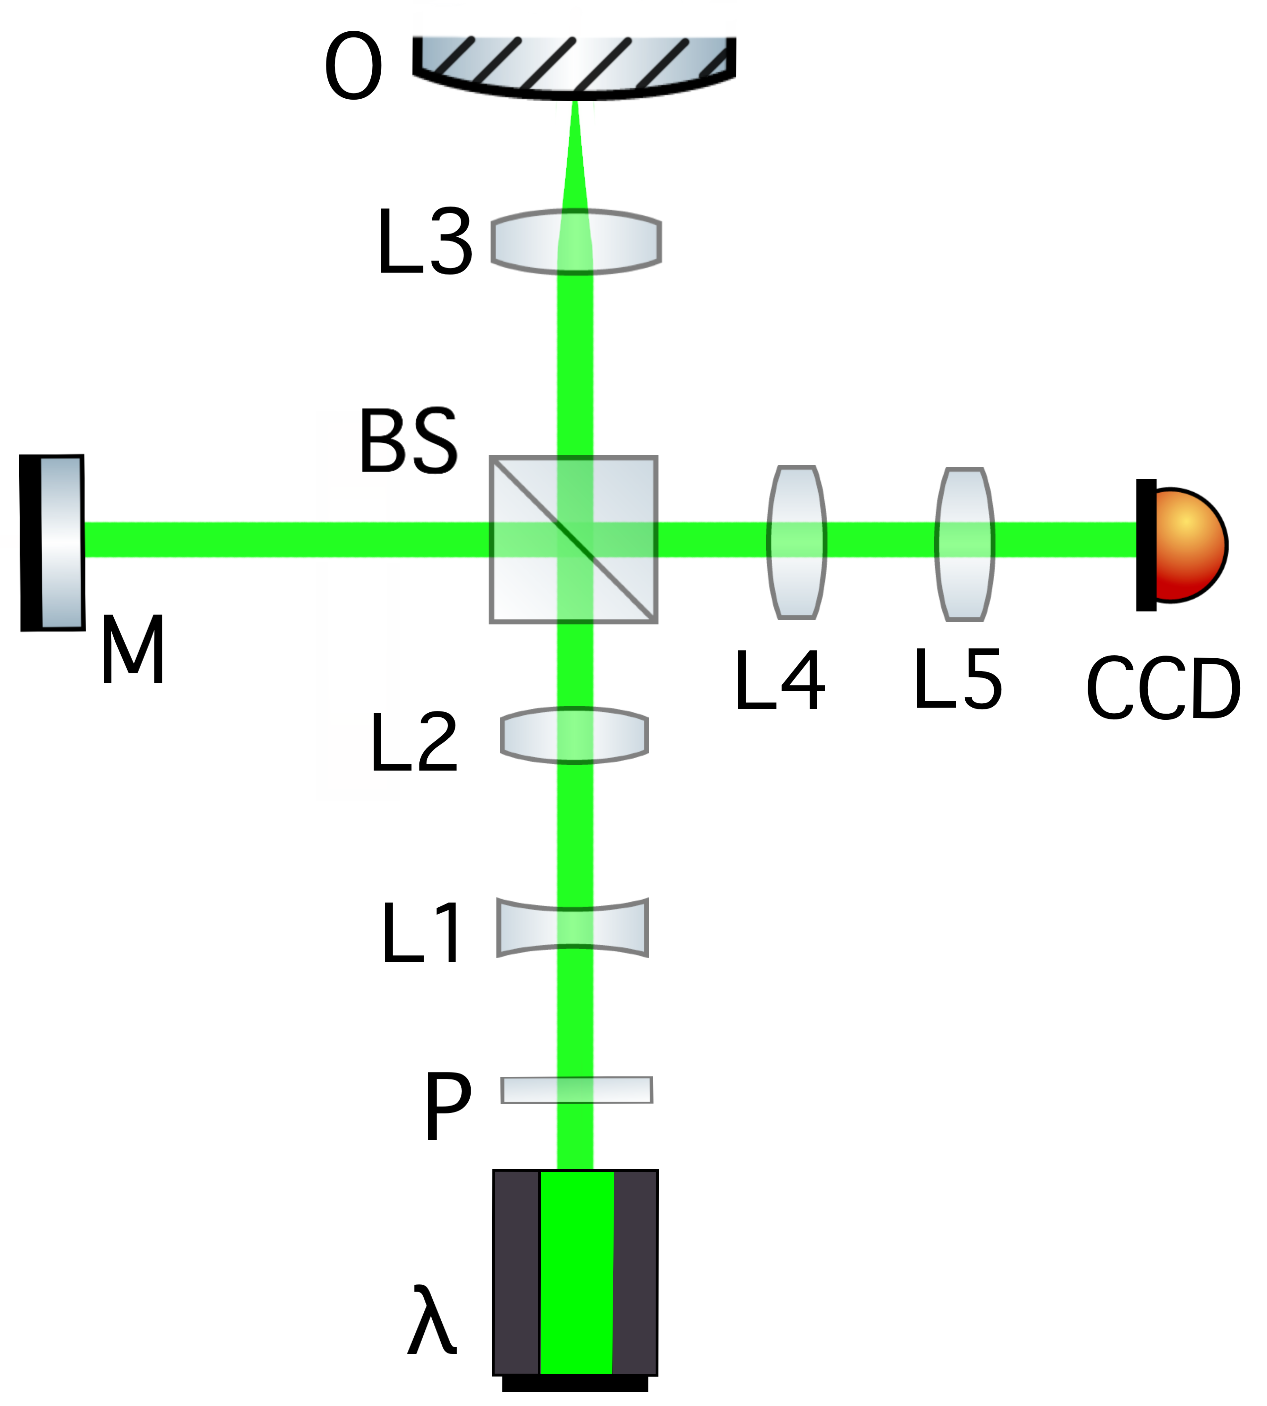
\includegraphics[width=\linewidth]{figs/interferometer_schematic.png}
\caption{Optical layout of the two-channel modified Michelson interferometer: $\lambda$ -- diode laser (532 nm); $P$ -- linear polariser; $L$ -- lenses; $L_3$ -- microscope objective; $M$ -- reference mirror ($\lambda/10$ flatness); $BS$ -- non-polarising beamsplitter; $O$ -- object on rotation stage; $CCD$ -- camera.}
\label{fig:layout}
\end{minipage}\hfill
\begin{minipage}[t]{0.48\linewidth}
\centering
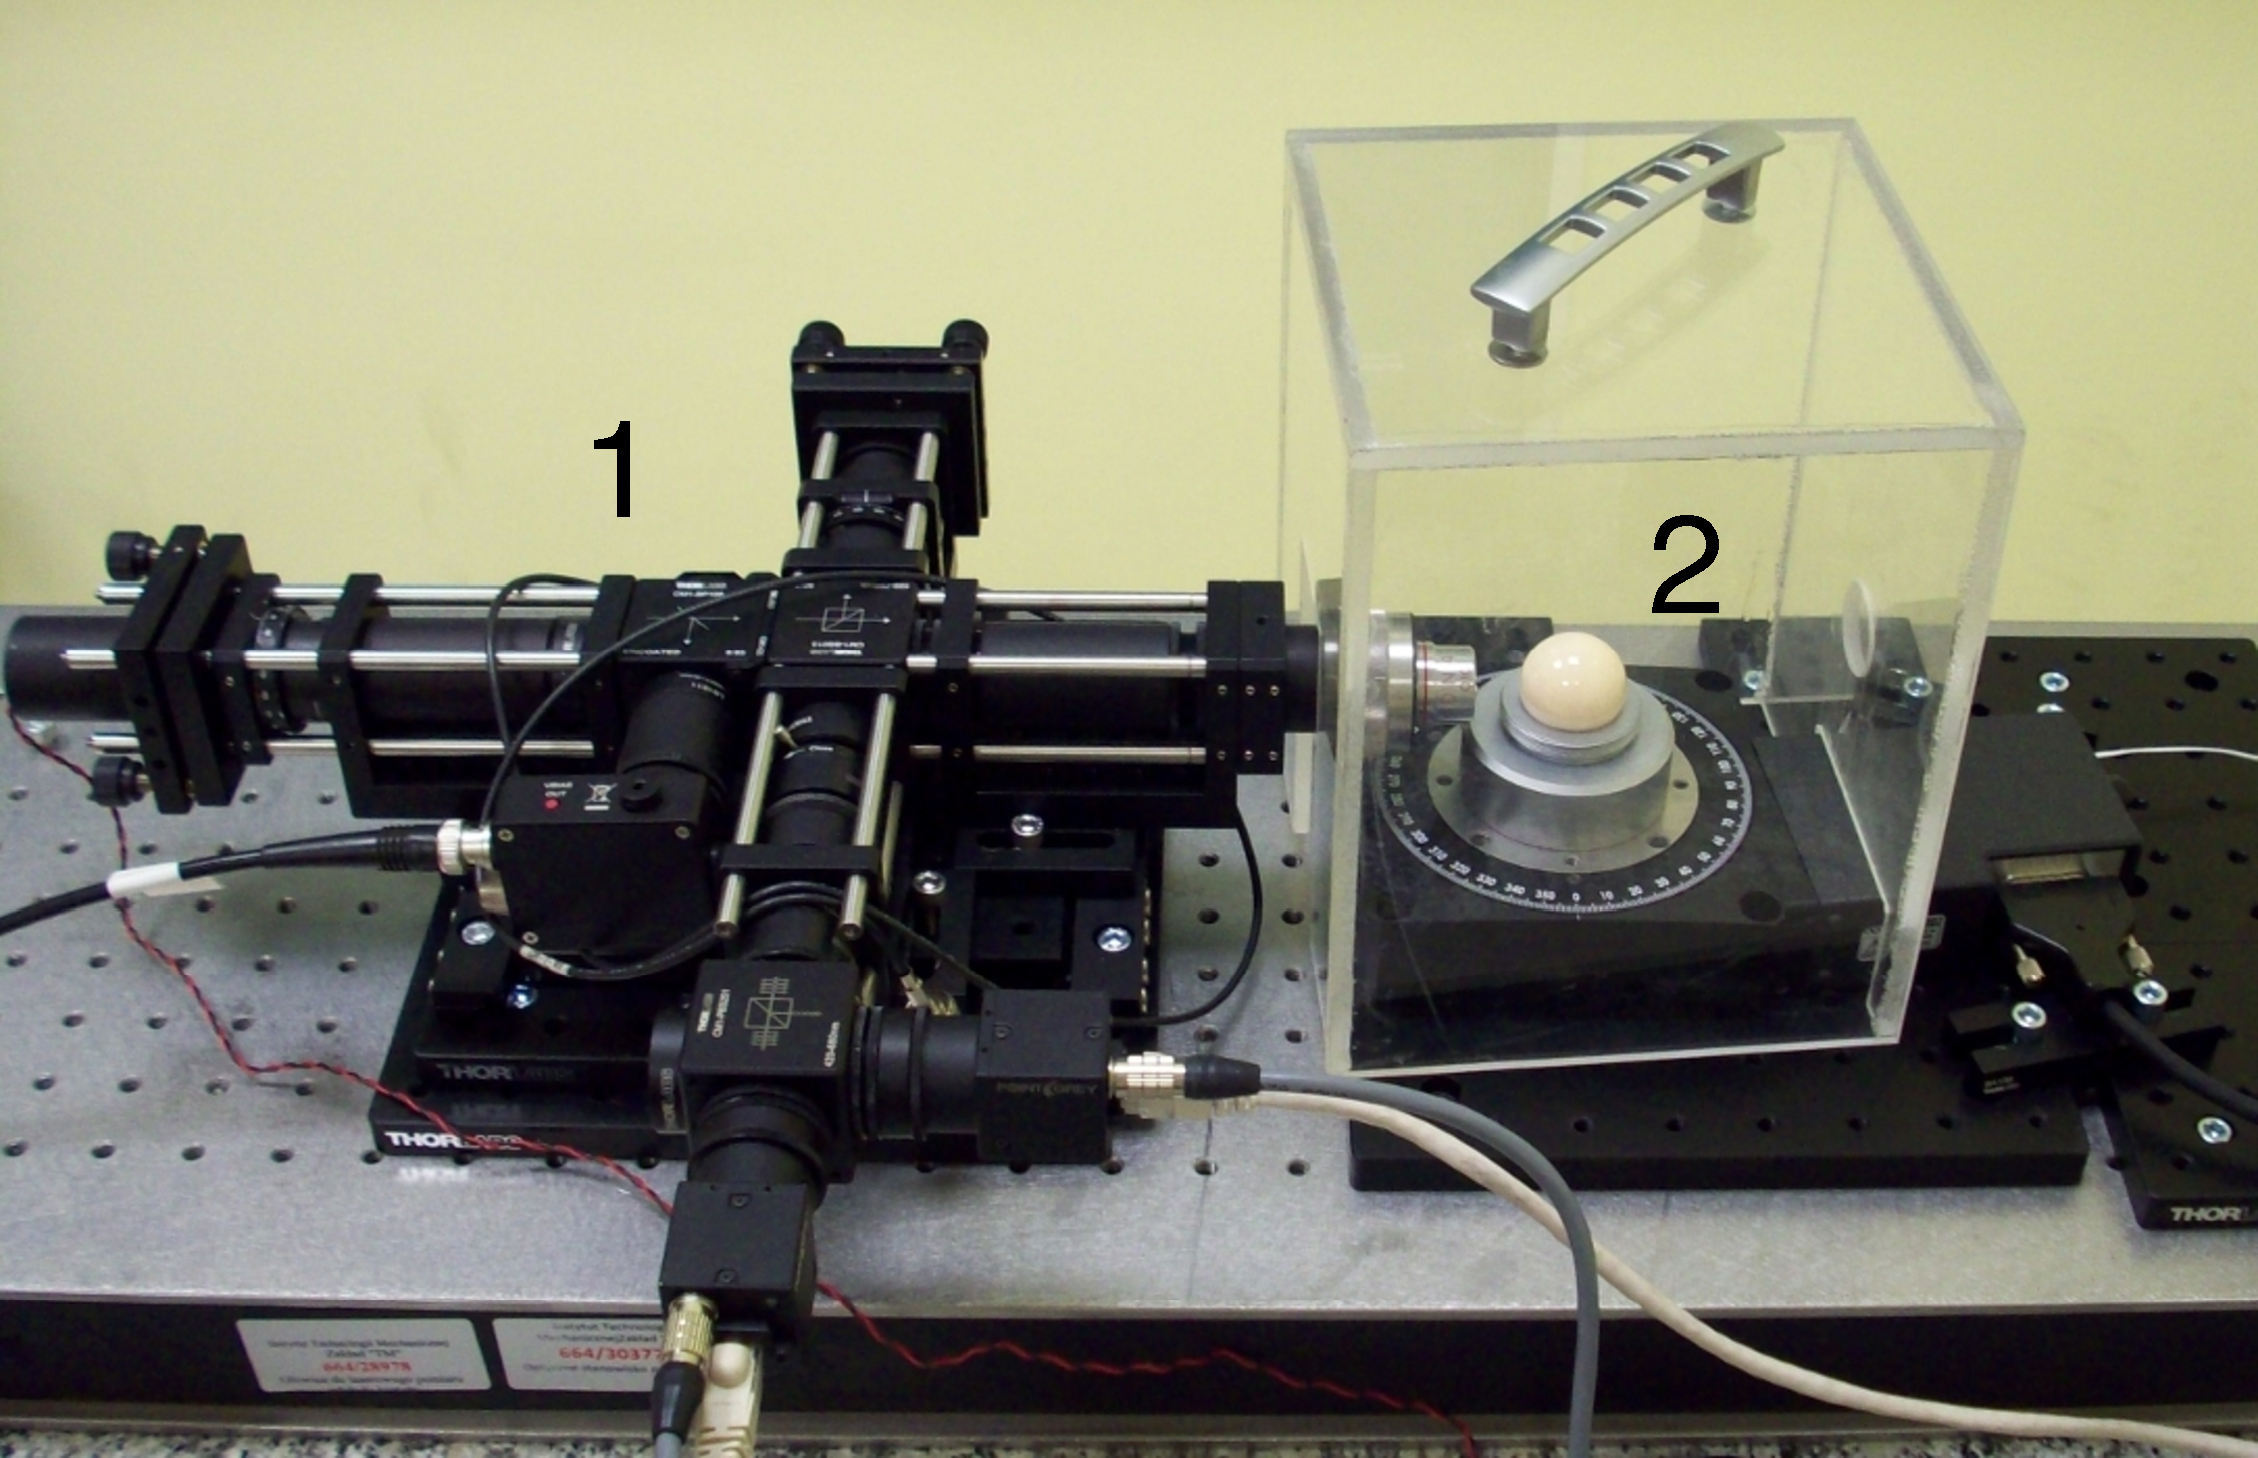
\includegraphics[width=\linewidth]{figs/100_2306.pdf}
\caption{The complete measurement system: (1)~modified Michelson interferometer in cage mounting, (2)~high-precision rotation stage with the artefact.}
\label{fig:tg_lab_setup1}
\end{minipage}
\end{figure}

The system was first tested with the JENOPTIK roundness standard FN~111 (photographs: Supplementary Fig.~S1) ($Al_2O_3$, \diameter~=~29.9588~mm)~\cite{JENOPTIK_ball}. A single-mode 4.5 mW diode laser with wavelength 532 nm was used as the light source. A current-stabilised supply powered the laser to obtain a stable wavelength~\cite{thorlabs_CPS532}. The laser beam passes through a polariser ($P$ in Fig.~\ref{fig:layout}) to set the polarisation of the light at $45^\circ$ to the setup plane, minimising the difference in reflectivity between the two channels.

Key components: achromatic lenses $L_{1,2,4,5}$, non-polarising beamsplitter $BS$, $\lambda/8$ liquid phase retarder, $\lambda/10$ reference mirror $M$, DIN-4 microscope objective $L_3$ (NA~0.10), polarising beamsplitter $PBS$, and two Gigabit Ethernet CCD cameras (640$\times$480 px, 120~fps).

The interferometer was built in a cage system for thermal, acoustic and mechanical stability. A plexiglass box shields the measurement object, and the structure is mounted on an area translation stage. A high-precision rotation stage (encoder accuracy 2.0~mdeg, typical wobble $\pm 12~\mu$rad, typical eccentricity $\pm 0.40~\mu$m; full specifications: Supplementary Table~S1) rotates the object. Both interferometer and stage are mounted on a honeycomb breadboard with vibration isolation.

Measurements were performed at night (23:00--05:00) to minimise building-activity disturbances. The setup was thermally and acoustically shielded (plexiglass box, wool blanket) and placed on a granite plate on layered wooden-polystyrene vibration isolation (photographs: Supplementary Fig.~S2). Five semiconductor temperature sensors ($\pm 0.2^\circ$C) monitored stability; the temperature near the reference and object arms remained stable to $\pm 0.2^\circ$C over six-hour acquisitions.

\subsection{Control System and Acquisition Workflow}
Cameras were controlled by FLIR SDK-based C programs and Bash scripts~\cite{FLIR_sdk}. Capture time was recorded per frame for angular-position verification. The rotation stage was controlled via USB ASCII commands~\cite{newport_esp_manual}; a 25~s settling delay ensured constant velocity before acquisition began. Object centring was performed manually using the two-camera phase-shifted configuration at $45^\circ$ rotation increments. Fringe evaluation used modified open-source R code~\cite{Meijer2018a,Ihaka1996}. Table~\ref{tab:meas_param} lists the acquisition parameters for both archives; five $400^\circ$ sweeps were recorded per artefact, with the $40^\circ$ overlap retained for profile-end comparison.

\begin{table}[ht]
\centering
\caption{Measurement and sampling parameters of the interferometric acquisition workflow.}
\label{tab:meas_param}
\begin{tabular}{lcc}
\toprule
Parameter & FN~111 & FN~101 \\
\midrule
Rotation speed, $\omega$ & 0.50 $^\circ$/s & 0.08 $^\circ$/s \\
CCD frame rate & 6 fps & 4 fps \\
Recorded sweeps, $n$ & 5 & 5 \\
Total frames, $N$ & 24,000 & 100,000 \\
Angular step, $\Delta\alpha=\omega/\mathrm{fps}$ & 0.083$^\circ$/frame & 0.020$^\circ$/frame \\
Frames per degree & 12 & 50 \\
Frames per useful $360^\circ$ & 4320 & 18,000 \\
Frames per recorded $400^\circ$ sweep & 4800 & 20,000 \\
Overlap per sweep & 40$^\circ$ / 480 frames & 40$^\circ$ / 2000 frames \\
Total acquisition time & 4000 s & 25,000 s \\
\bottomrule
\end{tabular}
\end{table}

The object was measured in one continuous five-sweep rotation without repositioning. Each recorded sweep spans $400^\circ$; successive useful $360^\circ$ segments are shifted by $40^\circ$, giving a natural between-sweep angular offset. The $40^\circ$ overlap region provides a model-free repeatability check: RMS height difference between consecutive sweeps is $12$~nm (FN~111) and $0.18~\mu$m (FN~101), consistent with Table~\ref{tab:metric_phase_reconstruction}.

\DIFaddbegin \DIFadd{The frame rates in Table~\ref{tab:meas_param} (6 and 4~fps) are far below the 120~fps capability of the cameras and merit comment. The angular step is set by the ratio $\Delta\alpha=\omega/\mathrm{fps}$, so angular resolution is governed jointly by rotation speed and frame rate; measurement time is governed by rotation speed alone. The rotation speeds (0.50 and 0.08~$^\circ$/s) were deliberately conservative: slow, constant-velocity rotation minimises dynamic excitation of the stage and keeps the fringe pattern quasi-static within each exposure, and the settling-time protocol (25~s before acquisition) assumes steady-state velocity. At these speeds, 6 and 4~fps already yield 12 and 50 frames per degree — an oversampling factor of roughly 300 and 1200 relative to the 15~UPR metrological bandwidth — so the frame rate was not the accuracy-limiting factor; increasing it at fixed rotation speed would only add redundant frames. Shorter total acquisition (4,000 and 25,000~s here) would instead require faster rotation with a proportionally higher frame rate, which is technically feasible with the present cameras up to 120~fps. Whether fringe contrast and stage stability are preserved at, say, a tenfold higher speed has not been tested; the trade-off between acquisition speed, vibration robustness, and per-frame phase-extraction quality is identified as a topic for future work, since measurement time is a critical parameter for industrial implementation.
}


\DIFaddend \section{Image Processing and Functional-Descriptor Method}

\subsection{Processing Pipeline}
The pipeline follows the radial excess-fraction method of a previous study~\cite{kucharski2025radial-0ca} with added sinusoidal refinement. Each interferogram $I_i(x,y)$ is decoded independently to a wrapped excess fraction $\epsilon_i$; the sequence is unwrapped chronologically, converted to nanometres ($z_i = \nu_i\lambda/2$), and reduced by the object-specific LSCI reference model. Sweep boundaries are retained for repeatability analysis.

\subsection{Step-by-Step Radial Phase Decoding}
For each interferogram $I_i(x,y)$, a radial intensity profile about the fringe centre is extracted and B-spline-smoothed; bright-ring maxima are detected in $D^2$ space, where circular-fringe theory gives $D_{ij}^{2}=c_i(j+\epsilon_i-1)$ for the $j$th ring of diameter $D_{ij}$. A linear fit $D_{ij}^{2}=\alpha_i j+\beta_i$ yields the wrapped excess fraction $\epsilon_i=(1+\beta_i/\alpha_i)\bmod 1$~\eqref{eq:epsilon_from_intercept}. Where the radial fringe signal permits ($R^2\geq0.65$, phase within 0.20 fringe of the ring-diameter estimate), a sinusoidal refinement is applied; otherwise the ring-diameter estimate is retained. The ordered series $\epsilon_i$ is unwrapped chronologically to a continuous fringe-order coordinate $\nu_i$, and the nanometre profile follows from $z_i=\nu_i\lambda/2$ with $\lambda=532$~nm (one fringe order $\equiv 266$~nm)~\eqref{eq:half_wavelength_conversion}.
\begin{equation}
D_{ij}^{2}=c_i(j+\epsilon_i-1),
\label{eq:ring_diameter_relation}
\end{equation}
\begin{equation}
\epsilon_i=\left(1+\frac{\beta_i}{\alpha_i}\right)\bmod 1.
\label{eq:epsilon_from_intercept}
\end{equation}
\begin{equation}
z_i=\nu_i\frac{\lambda}{2}, \qquad \lambda=532~\mathrm{nm}.
\label{eq:half_wavelength_conversion}
\end{equation}

\subsection{Topography Profile, Reference Removal and Eccentricity Reduction}
\label{sec:topography}
After phase-to-height conversion, the roundness profile is extracted following ISO~12181-1~\cite{ISO12181-1} (which supersedes the withdrawn ISO~4291\DIFaddbegin \DIFadd{~\mbox{%DIFAUXCMD
\cite{ISO4291}}\hskip0pt%DIFAUXCMD
}\DIFaddend ). For each $360^\circ$ segment, a least-squares reference circle (LSCI) is fitted to the angular height profile $z_i = h(\theta_i)$ in Cartesian coordinates:
\begin{equation}
(x_i, y_i) = \big((R_0 + z_i)\cos\theta_i,\; (R_0 + z_i)\sin\theta_i\big),
\end{equation}
where $R_0 = 14.9794$~mm is the nominal radius of the JENOPTIK FN~111. The LSCI centre $(x_c, y_c)$ minimises $\sum_i [\sqrt{(x_i-x_c)^2+(y_i-y_c)^2} - R_0]^2$, yielding the centred radial residuals $\rho_i$. The LSCI fit is numerically equivalent to removing the first harmonic of the angular profile, but it provides the formal ISO~4291 reference circle required for roundness metrology. After LSCI centring, a phase-correct Gaussian low-pass profile filter with 50\% transmission at 15 undulations per revolution (UPR) is applied to the residual profile, consistent with the filter specification used for the tactile reference measurements and with the Gaussian profile filter defined in ISO~16610-21\DIFaddbegin \DIFadd{:2025~\mbox{%DIFAUXCMD
\cite{ISO16610-21}}\hskip0pt%DIFAUXCMD
}\DIFaddend . All classical and gradient-based descriptors are computed from this LSCI-centred, Gaussian-filtered residual $\rho_i^{(\mathrm{filt})}$.

For the JENOPTIK magnification standard FN~101, the same processing chain is applied: a linear trend is removed from the unwrapped phase sequence before height conversion (Sec.~\ref{sec:discussion_drift}), the LSCI reference circle is fitted to the angular profile, and the Gaussian low-pass filter (50\% at 15~UPR) is applied. Although both artefacts are processed through identical filtering steps, the 15~UPR cutoff corresponds to different spatial wavelengths on the circumference: $2\pi \times 14.9794~\mathrm{mm}/15 = 6.27$~mm for the FN~111 ($\varnothing=29.9588$~mm) and $2\pi \times 15~\mathrm{mm}/15 = 6.28$~mm for the FN~101 ($\varnothing \approx 30$~mm) — effectively identical. The angular sampling differs substantially ($0.083^\circ$ vs.\ $0.020^\circ$, Table~\ref{tab:meas_param}), but the Gaussian filter sigma is set by the UPR cutoff, not by the sampling interval, so the filtered profiles are directly comparable.

\subsection{Classical Profile and Roundness Metrics}
All classical quantities are evaluated on nanometre residuals, not on raw intensities, following the profile method of ISO~\DIFaddbegin \DIFadd{21920-2~\mbox{%DIFAUXCMD
\cite{ISO21920-2}}\hskip0pt%DIFAUXCMD
, which supersedes the earlier ISO~}\DIFaddend 4287~\cite{ISO4287}\DIFaddbegin \DIFadd{; the amplitude-parameter definitions used here are common to both documents, and ISO~4287 is retained as a secondary reference because the tactile comparison data and the previous study~\mbox{%DIFAUXCMD
\cite{kucharski2025radial-0ca} }\hskip0pt%DIFAUXCMD
predate the transition}\DIFaddend . Areal parameters (ISO~25178~\cite{ISO25178}) are not reported because the single-image radial extraction does not produce a calibrated areal height map. For a residual profile or vector of residual pixels $p$, the reported profile-style roughness descriptors are
\begin{equation}
R_a=\frac{1}{M}\sum_{j=1}^{M}|p_j-\bar{p}|, \qquad
R_q=\left[\frac{1}{M}\sum_{j=1}^{M}(p_j-\bar{p})^2\right]^{1/2},
\end{equation}
and
\begin{equation}
R_z=\max_j(p_j-\bar{p})-\min_j(p_j-\bar{p}).
\end{equation}
\DIFaddbegin \DIFadd{As implemented, this quantity is the global peak-to-valley height of the full evaluation profile, corresponding to the total-height parameter ($Rt$ in ISO~21920-2 terms) rather than the section-averaged $Rz$; the symbol $R_z$ is retained for continuity with the previous study~\mbox{%DIFAUXCMD
\cite{kucharski2025radial-0ca}}\hskip0pt%DIFAUXCMD
. This implementation detail is relevant to the interpretation of Table~\ref{tab:metric_phase_reconstruction} (Sec.~\ref{sec:rz_ront}).
}\DIFaddend The profile skewness $R_{sk}$ and kurtosis $R_{ku}$ — ISO~\DIFdelbegin \DIFdel{4287 }\DIFdelend \DIFaddbegin \DIFadd{21920-2 }\DIFaddend shape parameters that characterise asymmetry and peakedness of the height distribution — are also reported:
\begin{equation}
R_{sk}=\frac{1}{R_q^3}\frac{1}{M}\sum_{j=1}^{M}(p_j-\bar{p})^3, \qquad
R_{ku}=\frac{1}{R_q^4}\frac{1}{M}\sum_{j=1}^{M}(p_j-\bar{p})^4.
\end{equation}
$R_{sk}=0$ for a symmetric distribution; $R_{sk}<0$ indicates a predominance of valleys over peaks. $R_{ku}=3$ for a normal distribution; $R_{ku}>3$ indicates a spikier (leptokurtic) profile. These are the only ISO~\DIFdelbegin \DIFdel{4287 }\DIFdelend \DIFaddbegin \DIFadd{21920-2 amplitude-distribution }\DIFaddend parameters that capture distribution shape beyond amplitude averages, and their inclusion allows a direct test of whether gradient-based descriptors provide information beyond even the best ISO shape parameters.
For the eccentricity-corrected ceramic angular profile $q_C(\theta)$,
\begin{equation}
RONt=\max_{\theta}q_C(\theta)-\min_{\theta}q_C(\theta), \qquad
RONq=\left[\frac{1}{2\pi}\int_0^{2\pi}q_C^2(\theta)\,d\theta\right]^{1/2}.
\end{equation}
These are profile/form quantities in nanometres. B-spline pre-smoothing (20 degrees of freedom, $\approx 18^\circ$ period) stabilises the LSCI fit; the subsequent Gaussian low-pass filter (50\% at 15~UPR, ISO~16610-21\DIFaddbegin \DIFadd{:2025}\DIFaddend ) defines the metrological bandwidth. All descriptors are computed from the same Gaussian-filtered residual.

\subsection{Functional Gradient-Based Descriptors}
The concept of a complete normed vector space originates from the foundational work of Banach~\cite{Banach1932}. For discrete profile data of finite length $N$, the vector space $\mathbb{R}^N$ equipped with any norm is a Banach space; the present work does not invoke infinite-dimensional completeness but draws on the taxonomy of $L^p$, Sobolev, and bounded-variation norms that Banach's framework systematised. For a centred residual profile $p(s)$ and $1\leq p<\infty$,
\begin{equation}
\|p\|_{p}=\left(\frac{1}{L}\int_0^L |p(s)|^p\,ds\right)^{1/p}, \qquad
\|p\|_{\infty}=\max_{s\in[0,L]}|p(s)|.
\end{equation}
The reported functional descriptors include $L^1$, $L^2$, $L^\infty$, the one-dimensional Sobolev $W^{1,2}$ seminorm and the bounded-variation (BV) total variation,
\begin{equation}
|p|_{W^{1,2}}=\left(\int_0^L\left|\frac{dp}{ds}\right|^2 ds\right)^{\!1/2}, \qquad TV(p)=\int_0^L \left|\frac{dp}{ds}\right|\,ds.
\end{equation}
In discrete form, for a uniformly sampled profile $p_j$ ($j=1,\dots,N$) with angular spacing $\Delta\alpha$,
\begin{equation}
|p|_{W^{1,2}} \approx \left(\Delta\alpha\sum_{j=1}^{N-1}\left(\frac{p_{j+1}-p_j}{\Delta\alpha}\right)^2\right)^{\!1/2}, \qquad
TV(p) \approx \sum_{j=1}^{N-1}|p_{j+1}-p_j|.
\end{equation}
Both $W^{1,2}$ and BV density carry sampling-interval dependence\DIFdelbegin \DIFdel{and require conversion to angular units (nm\,deg$^{-1/2}$ and nm\,deg$^{-1}$, respectively) for cross-instrument comparison}\DIFdelend ; ``nm\,sample$^{-1}$'' is retained \DIFaddbegin \DIFadd{in the result tables }\DIFaddend for the fixed-acquisition setup\DIFdelbegin \DIFdel{.
}\DIFdelend \DIFaddbegin \DIFadd{, and a standardised angular-unit convention for cross-instrument comparison is defined in Sec.~\ref{sec:angular_units}.
}\DIFaddend 

The curvature RMS (root-mean-square of the discrete second derivative; reported in Supplementary Table~S2) carries a $(\Delta\alpha)^{-2}$ sampling dependence and should not be compared across instruments with different angular resolution.

\subsection{\DIFdelbegin \DIFdel{Repeatability Uncertainty}\DIFdelend \DIFaddbegin \DIFadd{Angular-Unit Convention for Sampling-Dependent Descriptors}\DIFaddend }
\DIFaddbegin \label{sec:angular_units}
\DIFadd{Gradient-based descriptors evaluated on discretely sampled profiles depend on the sampling interval: the discrete total variation of an unfiltered profile grows as the sampling grid refines (noise contributes gradient content at every scale), so raw per-sample values are instrument-specific. For meaningful cross-instrument comparison the following convention is proposed and used here.
}

\begin{enumerate}
\item \textbf{\DIFadd{Band-limit first.}} \DIFadd{The profile is filtered with a declared phase-correct Gaussian profile filter (ISO~16610-21:2025) at a stated cutoff in undulations per revolution (here 50\% transmission at 15~UPR). After band-limiting, the profile derivative is bounded and the discrete sums converge to the continuous integrals as $\Delta\alpha\to 0$; the descriptor then characterises the declared bandwidth rather than the sampling grid.
}\item \textbf{\DIFadd{Sample adequately.}} \DIFadd{The angular sampling must resolve the declared bandwidth with margin; at least ten samples per cutoff undulation are recommended. Here the FN~111 and FN~101 profiles carry $\approx$290 and $\approx$1200 samples per 15-UPR undulation, so discretisation error is negligible.
}\item \textbf{\DIFadd{Report in angular units.}} \DIFadd{The BV density is reported as total variation per unit angle, $\mathrm{BV}_\theta = TV(p)/\Theta$ in nm\,deg$^{-1}$ ($\Theta=360^\circ$), and the gradient content as the RMS angular gradient $g_{\mathrm{rms}} = [\frac{1}{N-1}\sum_j ((p_{j+1}-p_j)/\Delta\alpha)^2]^{1/2}$ in nm\,deg$^{-1}$, together with the filter cutoff. For comparison across artefacts or instruments of }\emph{\DIFadd{different diameter}}\DIFadd{, the angular unit is additionally converted to an arc-length unit by dividing by the arc length per degree, $\pi D/360$; the BV density is then $\mathrm{BV}_s = TV(p)/(\pi D)$ in nm\,mm$^{-1}$. The arc-length form is the diameter-independent unit and is the one recommended for cross-instrument reporting, since nm\,deg$^{-1}$ still scales with the circumference of the specific artefact.
}\end{enumerate}

\DIFadd{A note on physical dimensions clarifies why this is necessary and is itself part of the answer to the redundancy question (Sec.~\ref{sec:critical}). Amplitude descriptors ($R_a$, $R_q$, $L^1$, $L^2$, $L^\infty$, $RONt$) have the dimension of length (nm) and are sampling-independent. Gradient descriptors are dimensionally distinct: BV density and the RMS gradient are height-per-length (nm\,mm$^{-1}$), i.e.\ dimensionless slopes, while the $W^{1,2}$ seminorm as defined here is height\,$\times$\,length$^{-1/2}$. This dimensional separation is the reason the gradient layer carries information that no amplitude parameter can encode, and also the reason its raw per-sample value must be qualified by a sampling and filter declaration.
}

\DIFadd{For the present data, the per-sample values in Table~\ref{tab:metric_phase_reconstruction} convert as follows. FN~111 ($\Delta\alpha=0.083^\circ$): BV density $0.263$~nm\,sample$^{-1}$ $\rightarrow$ $3.2$~nm\,deg$^{-1}$ $\rightarrow$ $12.1$~nm\,mm$^{-1}$; RMS gradient $0.310$~nm\,sample$^{-1}$ $\rightarrow$ $3.7$~nm\,deg$^{-1}$ $\rightarrow$ $14.2$~nm\,mm$^{-1}$. FN~101 ($\Delta\alpha=0.020^\circ$): BV density $6.58$~nm\,sample$^{-1}$ $\rightarrow$ $329$~nm\,deg$^{-1}$ $\rightarrow$ $1.26~\mu$m\,mm$^{-1}$; RMS gradient $8.76$~nm\,sample$^{-1}$ $\rightarrow$ $438$~nm\,deg$^{-1}$ $\rightarrow$ $1.67~\mu$m\,mm$^{-1}$, all at the 15-UPR cutoff. The two artefacts have almost identical circumference ($\pi D \approx 94.1$ and $94.2$~mm), so the large difference in arc-length gradient content ($12$ versus $1257$~nm\,mm$^{-1}$) reflects a genuine difference in surface variation rather than a unit artefact. Because each conversion is a fixed multiplicative factor for a given acquisition, relative uncertainties and relative defect responses are identical in every unit system. Adoption of gradient descriptors in reference software for roundness evaluation would require exactly this pair of declarations --- filter cutoff and arc-length units --- which parallels the established practice of declaring the filter for $RONt$.
}

\DIFadd{An empirical demonstration that this convention removes the sampling dependence is obtained by decimating the FN~111 residual of session A from 12 to 1 samples per degree (a factor of 12) and recomputing the descriptors with the 15-UPR Gaussian filter matched to each sampling. The band-limited BV density and RMS gradient change by less than 0.5\% across the full decimation range, whereas the unfiltered total variation drops by a factor of 3.3 over the same range. This confirms that the declared filter --- not the sampling grid --- defines the descriptor value, and shows that the recommendation of at least ten samples per cutoff undulation is conservative: even 24 samples per cutoff undulation reproduce the band-limited values to within 0.5\%.
}

\subsection{\DIFadd{Uncertainty Evaluation}}
\label{sec:uncertainty}
\DIFaddend Each dataset contains five $400^\circ$ sweeps recorded in a single continuous rotation without stopping or repositioning. The five useful $360^\circ$ segments are extracted from this continuous sequence; because each recorded sweep spans $400^\circ$, successive useful revolutions are shifted by $40^\circ$ on the object. These segments are not strictly independent — they share the same continuous-run conditions (laser warm-up state, stage-bearing temperature, ambient drift). The standard deviation across sweeps therefore reflects within-run repeatability rather than between-run reproducibility. For a descriptor $X$ evaluated on each sweep, the mean value is $\bar{X}$ and the within-run standard uncertainty is estimated as
\begin{equation}
u_{\mathrm{within}}(X)=\frac{s_X}{\sqrt{n}}, \qquad n=5,
\end{equation}
where $s_X$ is the sample standard deviation across the five sweeps. The reported expanded uncertainty is
\begin{equation}
U_{95}(X)=t_{0.975,n-1}\,u_{\mathrm{within}}(X).
\end{equation}
With $n=5$, $t_{0.975,4}=2.776$; the $\chi^2_4$-based 95\% CI for the standard deviation spans $[0.6s_X,\,2.9s_X]$, so $U_{95}$ is indicative rather than definitive. Because the five segments share continuous-run conditions (laser state, stage temperature, ambient drift), the $1/\sqrt{n}$ factor in $u_{\mathrm{within}}$ may underestimate the true uncertainty of the mean; all reported uncertainties are \emph{lower bounds}. \DIFdelbegin \DIFdel{A full GUM-compliant budget (}\DIFdelend \DIFaddbegin \DIFadd{An indicative }\DIFaddend type-B \DIFdelbegin \DIFdel{terms: laser wavelength stability, refractive-index variations, Abbe error~\mbox{%DIFAUXCMD
\cite{NewportCorporation:2018vk}}\hskip0pt%DIFAUXCMD
, camera nonlinearity, form-removal uncertainty)is beyond the present scope}\DIFdelend \DIFaddbegin \DIFadd{budget for the principal systematic terms is given in Sec.~\ref{sec:typeB}; a complete GUM-compliant budget~\mbox{%DIFAUXCMD
\cite{JCGM100} }\hskip0pt%DIFAUXCMD
with experimentally characterised input distributions, and a between-run reproducibility study with independent setups, thermal cycles, and physical re-centring of the artefact, remain future work (Sec.~\ref{sec:future})}\DIFaddend . With $n=5$ sweeps and the observed within-run variability, the minimum detectable relative difference between two descriptors (80\% power, $\alpha=0.05$, two-sided paired $t$-test) is approximately $30\%$ for the FN~111 and $5\%$ for the FN~101, consistent with the exploratory character of the descriptor comparison. A per-sweep trend of FN~111 $RONt$ values gives a slope of $8.4\pm4.1$~nm\,sweep$^{-1}$ ($p=0.12$), consistent with zero drift, though the sweep-to-sweep scatter cautions that $U_{95}$ may underestimate long-term reproducibility.

\DIFaddbegin \subsection{\DIFadd{Indicative Type-B Uncertainty Budget}}
\label{sec:typeB}
\DIFadd{Although a complete GUM budget requires between-run data that the present single-rotation acquisition cannot supply, the principal type-B contributions can be bounded from component specifications and pipeline properties. Table~\ref{tab:typeB} summarises the estimates for the FN~111 $RONt$ evaluation; the same relative arguments apply to the FN~101.
}

\emph{\DIFadd{Laser wavelength stability.}} \DIFadd{The height scale $z=\nu\lambda/2$ inherits the relative wavelength error: a $\pm1$~nm tolerance on the 532~nm diode module (rectangular distribution) gives a relative standard uncertainty of $0.11\%$, i.e.\ $0.3$~nm on $RONt=278$~nm (and $46$~nm on the FN~101 $RONt=42.07~\mu$m, within its $\pm0.48~\mu$m repeatability interval). Wavelength error acts as a pure scale factor and cannot create or mask localised features.
}

\emph{\DIFadd{Refractive index of air.}} \DIFadd{The in-air wavelength varies with temperature and pressure by $\sim10^{-6}$ per $1^\circ$C or 3~hPa; with the observed $\pm0.2^\circ$C stability the contribution is below $10^{-5}$ relative, i.e.\ $<0.01$~nm. Negligible.
}

\emph{\DIFadd{Abbe error and stage wobble.}} \DIFadd{The specified axis wobble ($\pm12~\mu$rad) enters through two mechanisms: a cosine-type radial error $R\theta_w^2/2\approx1$~pm, and a lateral beam walk $R\theta_w\approx0.18~\mu$m on the circumference, equivalent to an angular mislocation of $0.0007^\circ$, which maps through the local band-limited gradient ($\approx3.2$~nm\,deg$^{-1}$, Sec.~\ref{sec:angular_units}) to $\approx0.002$~nm. Both are negligible after LSCI first-harmonic removal.
}

\emph{\DIFadd{Camera nonlinearity and EFM localisation.}} \DIFadd{Intensity nonlinearity perturbs the radial fringe-peak positions; its effect is bounded empirically by the per-frame excess-fraction uncertainty of $\pm0.05$ fringe ($13$~nm). The 15-UPR band limit averages $\approx290$ frames per resolved undulation, reducing the per-point contribution to $\approx0.8$~nm and the peak-to-valley contribution to $\approx1.1$~nm.
}

\emph{\DIFadd{Long-term drift and phase noise floor (measured).}} \DIFadd{An independent static stability session, recorded with the same interferometer, camera settings and frame count as the FN~111 acquisition (24,000 frames over 4,000~s) but with the object not rotating, provides a direct experimental bound on slow instrument drift under realistic laboratory conditions. The decoded excess-fraction sequence spans only $98$~nm over the full session, with an end-to-end linear drift of $-82$~nm ($-1.1$~nm\,min$^{-1}$), i.e.\ $\approx15$~nm over one 800~s sweep-equivalent interval; after linear detrending the residual has $9.4$~nm standard deviation ($45$~nm peak-to-valley), and the frame-to-frame phase noise floor is $2.1$~nm ($0.008$ fringe). Two conclusions follow. First, the measured static noise floor is well below the conservative $\pm0.05$-fringe EFM bound used above, confirming that bound as conservative. Second, the slow drift maps predominantly to low harmonic orders of the angular profile, where it is largely absorbed by the LSCI first-harmonic removal, and its sweep-to-sweep manifestation is already contained in the type-A scatter; the drift bound is therefore reported as an informative constraint rather than added in quadrature.
}

\emph{\DIFadd{Form removal.}} \DIFadd{The LSCI reference (first-harmonic removal) is exact only in the lima\c{c}on approximation; the second-order term $a^2/(2R)$ for residual centring eccentricity $a$ leaks into the second harmonic of the residual. Manual centring leaves $a$ of the order of tens of micrometres (the shared first-harmonic model of Sec.~\ref{sec:eccentricity}, with its 63~nm/0.18\% per-sweep amplitude variation, implies $a\approx35~\mu$m); for $a=15$--$35~\mu$m the term evaluates to $7$--$41$~nm. Because this contribution is common to all five sweeps, it does not appear in the type-A scatter and must be carried as a bounded systematic term. Its magnitude is consistent with the $34$~nm difference between the optical $RONt$ ($278\pm22$~nm) and the certified tactile value ($244\pm52$~nm), a difference that the $E_n=0.61$ comparison shows to be within the combined uncertainties.
}

\begin{table}[htbp]
\centering
\footnotesize
\caption{\DIFaddFL{Indicative type-B uncertainty budget for the FN~111 $RONt$ evaluation. Random contributions are standard uncertainties combined in quadrature with the type-A term; the form-removal term is a bounded systematic (bias) contribution common to all sweeps and is reported separately.}}
\label{tab:typeB}
\begin{tabular}{p{0.42\textwidth}p{0.30\textwidth}p{0.17\textwidth}}
\toprule
\DIFaddFL{Source }& \DIFaddFL{Basis }& \DIFaddFL{Contribution to $RONt$ }\\
\midrule
\DIFaddFL{Within-run repeatability (type A) }& \DIFaddFL{$s/\sqrt{5}$, five sweeps }& \DIFaddFL{$7.9$~nm }\\
\DIFaddFL{Laser wavelength ($\pm1$~nm, rect.) }& \DIFaddFL{module specification }& \DIFaddFL{$0.3$~nm }\\
\DIFaddFL{Air refractive index ($\pm0.2^\circ$C) }& \DIFaddFL{Edl\'{e}n-type sensitivity }& \DIFaddFL{$<0.01$~nm }\\
\DIFaddFL{Abbe error / axis wobble ($\pm12~\mu$rad) }& \DIFaddFL{stage specification, geometry }& \DIFaddFL{$<0.01$~nm }\\
\DIFaddFL{Camera nonlinearity / EFM localisation }& \DIFaddFL{$\pm0.05$ fringe per frame, band-limited averaging }& \DIFaddFL{$1.1$~nm }\\
\DIFaddFL{Long-term drift (measured, static session) }& \DIFaddFL{$-1.1$~nm\,min$^{-1}$; $\leq15$~nm per sweep }& \DIFaddFL{informative bound$^{\dagger}$ }\\
\midrule
\DIFaddFL{Combined standard uncertainty $u_c$ (random) }& \DIFaddFL{quadrature }& \DIFaddFL{$8.0$~nm }\\
\DIFaddFL{Expanded $U_{95}$ (random, $t_{0.975,4}$) }& & \DIFaddFL{$22$~nm }\\
\midrule
\DIFaddFL{Form removal (lima\c{c}on second order) }& \DIFaddFL{$a^2/(2R)$, $a=15$--$35~\mu$m }& \DIFaddFL{$\leq41$~nm (syst.\ bound) }\\
\bottomrule
\end{tabular}

\smallskip
{\footnotesize \DIFaddFL{$^{\dagger}$Measured in an independent static session (Sec.~\ref{sec:typeB}); manifested in the type-A scatter and largely removed with the first harmonic, hence not added in quadrature.}}
\end{table}

\DIFadd{The quadrature combination is dominated by the type-A term, so the reported $U_{95}$ values are essentially unchanged by the enumerated random type-B terms; the budget nevertheless shows that the leading risks are the form-removal systematic and the between-run effects bounded in Sec.~\ref{sec:between_run}, not the enumerated instrument terms.
}

\subsection{\DIFadd{Between-Run Reproducibility of Independent Sessions}}
\label{sec:between_run}
\DIFadd{Two further independent acquisition sessions of the FN~111 were processed through the identical pipeline and descriptor computation (per-sweep LSCI-centred residual, circular Gaussian low-pass filter at 15~UPR) to assess between-run reproducibility with the archived material. The primary archive reported in Tables~\ref{tab:meas_param} and~\ref{tab:metric_phase_reconstruction} is denoted session A. Session B (0.50$^\circ$/s, 6~fps, 24,000 frames) repeats its acquisition parameters; session C (0.64$^\circ$/s, 8~fps, 25,000 frames, 0.08$^\circ$/frame) uses a different rotation speed and frame rate at nearly the same angular sampling. Sessions B and C were recorded on different days with the artefact re-mounted and re-centred. Table~\ref{tab:between_run} reports the relative between-session differences and the $E_n$ compatibility statistic, $E_n=|\Delta|/(2\sqrt{u_A^2+u_B^2})$, with the standard uncertainties of the per-sweep means ($n=5$).
}

\begin{table}[htbp]
\centering
\footnotesize
\caption{\DIFaddFL{Between-session comparison for the FN~111. Session A is the primary archive reported in Tables~1--3; sessions B and C are independent repeat acquisitions (B: same parameters; C: 0.64$^\circ$/s, 8~fps) with the artefact re-mounted and re-centred. Relative differences and $E_n$ compatibility values are reported; $E_n<1$ indicates agreement within the combined standard uncertainties of the per-sweep means.}}
\label{tab:between_run}
\begin{tabular}{lcc|cc}
\toprule
& \multicolumn{2}{c}{B vs.\ A} & \multicolumn{2}{c}{C vs.\ A} \\
\DIFaddFL{Descriptor }& \DIFaddFL{rel.\ diff. }& \DIFaddFL{$E_n$ }& \DIFaddFL{rel.\ diff. }& \DIFaddFL{$E_n$ }\\
\midrule
\DIFaddFL{$R_a$ }& \DIFaddFL{$-2.4\%$ }& \DIFaddFL{$0.35$ }& \DIFaddFL{$+7.0\%$ }& \DIFaddFL{$1.45$ }\\
\DIFaddFL{$R_q$ }& \DIFaddFL{$-2.0\%$ }& \DIFaddFL{$0.23$ }& \DIFaddFL{$+8.8\%$ }& \DIFaddFL{$1.51$ }\\
\DIFaddFL{$RONt$ }& \DIFaddFL{$-2.9\%$ }& \DIFaddFL{$0.23$ }& \DIFaddFL{$+12.3\%$ }& \DIFaddFL{$1.16$ }\\
\DIFaddFL{$L^{\infty}$ }& \DIFaddFL{$-0.1\%$ }& \DIFaddFL{$0.00$ }& \DIFaddFL{$+11.6\%$ }& \DIFaddFL{$0.79$ }\\
\DIFaddFL{BV density }& \DIFaddFL{$-4.0\%$ }& \DIFaddFL{$0.99$ }& \DIFaddFL{$+4.4\%$ }& \DIFaddFL{$1.25$ }\\
\DIFaddFL{$W^{1,2}$ grad. }& \DIFaddFL{$-3.8\%$ }& \DIFaddFL{$0.88$ }& \DIFaddFL{$+4.6\%$ }& \DIFaddFL{$1.40$ }\\
\bottomrule
\end{tabular}
\end{table}

\DIFadd{For session B, every descriptor agrees with session A within its combined uncertainty ($|E_n|<1$): the amplitude parameters differ by less than 3\% and the gradient descriptors by about 4\% (BV density, $E_n=0.99$, is the largest), showing that BV density and the $W^{1,2}$ seminorm are between-run stable to the same order as the classical parameters under identical acquisition parameters. For session C, the amplitude descriptors differ by 7--12\% ($E_n$ up to 1.5); the $RONt$ difference of $42$~nm is comparable to the $\leq41$~nm form-removal bound of Sec.~\ref{sec:typeB}, indicating that the dominant between-session variation arises from re-centring (first-harmonic leakage) rather than from the change of rotation speed or frame rate. The gradient descriptors change by $+4\%$ (per-sample) to $+9\%$ (angular units), tracking the shared amplitude change with no sampling-induced anomaly. Together with the static-session drift bound (Sec.~\ref{sec:typeB}), these results establish the first quantitative between-run stability statement for the gradient-based descriptors; a full multi-session campaign remains future work (Sec.~\ref{sec:future}).
}

\DIFaddend \subsection{Computational Implementation}
The reconstruction workflow (\path{scripts/reconstruct_radial_profile_sequence.py}) decodes $\epsilon_i$ from each interferogram, unwraps the sequence, converts to nanometres, applies LSCI fitting and Gaussian low-pass filtering (50\% at 15~UPR, ISO~16610-21\DIFaddbegin \DIFadd{:2025}\DIFaddend ), and exports CSV/JSON metrics with sweep-repeatability uncertainty. Vector PDF figures document each processing stage. The pipeline is invoked as \path{PYTHONPATH=src .venv/bin/python scripts/reconstruct_radial_profile_sequence.py} with dataset-specific parameters (full command in the data repository). Per-image excess-fraction decoding and unwrapping require approximately 0.5~ms per frame (measured on an Intel Core i7-9700K, single-threaded Python~3.9), so the full 124,000-frame archive processes in under two minutes on consumer hardware.

\section{Results}

The results follow the updated radial sequence route only. Each raw image is first decoded to a wrapped excess fraction from its radial fringe pattern. The ordered excess-fraction series is then unwrapped in chronological order, converted to nanometres, and corrected for eccentricity. Finally, classical profile/roundness descriptors and functional gradient-based descriptors are computed from the same nanometre residual profiles.

\subsection{Radial Phase Decoding and Nanometre Profile Reconstruction}
The FN~111 folder contained 24,000 interferograms and the steel folder contained 100,000 interferograms. The reported run used full-resolution images, the central radial aperture of 240 px, B-spline-smoothed peak detection, continuity-aware EFM peak-subset tracking and an EFM prominence threshold of 0.04 of the radial fringe-signal range. All five recorded sweeps were processed.

Figs.~S3--S6 (single-image EFM and sequence processing steps) are provided in the Supplementary Materials.

\subsection{Roughness, Roundness and Functional Descriptors}
Table~\ref{tab:metric_phase_reconstruction} gives the numerical comparison after LSCI reference circle and Gaussian low-pass filtering (50\% at 15~UPR). Both artefacts are processed through the same filtering chain. Each descriptor is reported as the full-sequence value together with the 95\% expanded type-A repeatability uncertainty estimated from the five sweeps. Per-sweep values for all descriptors are provided in Supplementary Table~S3.

\begin{table}[htbp]
\centering
\footnotesize
\setlength{\tabcolsep}{4pt}
\caption{Full-resolution radial EFM reconstruction from raw interferograms (LSCI + Gaussian low-pass, 50\% at 15~UPR, ISO~16610-21\DIFaddbeginFL \DIFaddFL{:2025}\DIFaddendFL ). Uncertainties are 95\% expanded within-run repeatability estimates from five sweeps ($n=5$, $t_{0.975,4}=2.776$). Units: nm for all descriptors except BV density and $W^{1,2}$ gradient (nm\,sample$^{-1}$). Certified $RONt$: FN~111 $244 \pm 52$~nm (Hommel Roundscan~535, $n=104$); FN~101 $41.94$~$\mu$m (form tester, $n=12$). The FN~101 certificate does not report an expanded uncertainty; therefore only the percentage difference is reported for this artefact rather than an $E_n$ score.}
\label{tab:metric_phase_reconstruction}
\begin{tabular}{lcc}
\toprule
Descriptor & FN~111 & FN~101 \\
\midrule
$R_a$ & \DIFdelbeginFL \DIFdelFL{$66.3 \pm 4.7$}\DIFdelendFL \DIFaddbeginFL \DIFaddFL{$(66.3 \pm 4.7)$}\DIFaddendFL \,nm & \DIFdelbeginFL \DIFdelFL{$8.525 \pm 0.115$}\DIFdelendFL \DIFaddbeginFL \DIFaddFL{$(8.525 \pm 0.115)$}\DIFaddendFL \,$\mu$m \\
$R_q$ & \DIFdelbeginFL \DIFdelFL{$77.6 \pm 5.0$}\DIFdelendFL \DIFaddbeginFL \DIFaddFL{$(77.6 \pm 5.0)$}\DIFaddendFL \,nm & \DIFdelbeginFL \DIFdelFL{$10.376 \pm 0.090$}\DIFdelendFL \DIFaddbeginFL \DIFaddFL{$(10.376 \pm 0.090)$}\DIFaddendFL \,$\mu$m \\
$R_z$ & \DIFdelbeginFL \DIFdelFL{$278 \pm 22$}\DIFdelendFL \DIFaddbeginFL \DIFaddFL{$(278 \pm 22)$}\DIFaddendFL \,nm & \DIFdelbeginFL \DIFdelFL{$42.07 \pm 0.48$}\DIFdelendFL \DIFaddbeginFL \DIFaddFL{$(42.07 \pm 0.48)$}\DIFaddendFL \,$\mu$m \\
$RONt$ & \DIFdelbeginFL \DIFdelFL{$278 \pm 22$}\DIFdelendFL \DIFaddbeginFL \DIFaddFL{$(278 \pm 22)$}\DIFaddendFL \,nm & \DIFdelbeginFL \DIFdelFL{$42.07 \pm 0.48$}\DIFdelendFL \DIFaddbeginFL \DIFaddFL{$(42.07 \pm 0.48)$}\DIFaddendFL \,$\mu$m \\
$RONq$ & \DIFdelbeginFL \DIFdelFL{$77.6 \pm 5.0$}\DIFdelendFL \DIFaddbeginFL \DIFaddFL{$(77.6 \pm 5.0)$}\DIFaddendFL \,nm & \DIFdelbeginFL \DIFdelFL{$10.376 \pm 0.090$}\DIFdelendFL \DIFaddbeginFL \DIFaddFL{$(10.376 \pm 0.090)$}\DIFaddendFL \,$\mu$m \\
$L^1$ mean & \DIFdelbeginFL \DIFdelFL{$66.3 \pm 4.7$}\DIFdelendFL \DIFaddbeginFL \DIFaddFL{$(66.3 \pm 4.7)$}\DIFaddendFL \,nm & \DIFdelbeginFL \DIFdelFL{$8.525 \pm 0.115$}\DIFdelendFL \DIFaddbeginFL \DIFaddFL{$(8.525 \pm 0.115)$}\DIFaddendFL \,$\mu$m \\
$L^2$ RMS & \DIFdelbeginFL \DIFdelFL{$77.6 \pm 5.0$}\DIFdelendFL \DIFaddbeginFL \DIFaddFL{$(77.6 \pm 5.0)$}\DIFaddendFL \,nm & \DIFdelbeginFL \DIFdelFL{$10.376 \pm 0.090$}\DIFdelendFL \DIFaddbeginFL \DIFaddFL{$(10.376 \pm 0.090)$}\DIFaddendFL \,$\mu$m \\
$L^{\infty}$ & \DIFdelbeginFL \DIFdelFL{$150 \pm 12$}\DIFdelendFL \DIFaddbeginFL \DIFaddFL{$(150 \pm 12)$}\DIFaddendFL \,nm & \DIFdelbeginFL \DIFdelFL{$21.97 \pm 0.42$}\DIFdelendFL \DIFaddbeginFL \DIFaddFL{$(21.97 \pm 0.42)$}\DIFaddendFL \,$\mu$m \\
BV total & \DIFdelbeginFL \DIFdelFL{$1.137 \pm 0.062$}\DIFdelendFL \DIFaddbeginFL \DIFaddFL{$(1.137 \pm 0.062)$}\DIFaddendFL \,$\mu$m & \DIFdelbeginFL \DIFdelFL{$118.4 \pm 6.2$}\DIFdelendFL \DIFaddbeginFL \DIFaddFL{$(118.4 \pm 6.2)$}\DIFaddendFL \,$\mu$m \\
BV density & \DIFdelbeginFL \DIFdelFL{$0.263 \pm 0.014$}\DIFdelendFL \DIFaddbeginFL \DIFaddFL{$(0.263 \pm 0.014)$}\DIFaddendFL \,nm\,sample$^{-1}$ & \DIFdelbeginFL \DIFdelFL{$6.58 \pm 0.35$}\DIFdelendFL \DIFaddbeginFL \DIFaddFL{$(6.58 \pm 0.35)$}\DIFaddendFL \,nm\,sample$^{-1}$ \\
$W^{1,2}$ grad. & \DIFdelbeginFL \DIFdelFL{$0.310 \pm 0.015$}\DIFdelendFL \DIFaddbeginFL \DIFaddFL{$(0.310 \pm 0.015)$}\DIFaddendFL \,nm\,sample$^{-1}$ & \DIFdelbeginFL \DIFdelFL{$8.76 \pm 0.43$}\DIFdelendFL \DIFaddbeginFL \DIFaddFL{$(8.76 \pm 0.43)$}\DIFaddendFL \,nm\,sample$^{-1}$ \\
\midrule
\multicolumn{3}{c}{\textit{ISO shape parameters}} \\
$R_{sk}$ (skewness) & $-0.09 \pm 0.04$ & $0.00 \pm 0.09$ \\
$R_{ku}$ (kurtosis) & $1.98 \pm 0.21$ & $2.51 \pm 0.08$ \\
\midrule
\multicolumn{3}{c}{\textit{Derived norm ratios}} \\
$L^4/L^1$ peakiness & $1.39 \pm 0.08$ & $1.53 \pm 0.03$ \\
\midrule
\multicolumn{3}{c}{\textit{External validation}} \\
$E_n$ score & $0.61$ & $<1$ ($0.3\%$ diff.; cf.~Fig.~S12) \\
\bottomrule
\end{tabular}
\end{table}

\DIFdelbegin \DIFdel{The numerical identity $RONt=R_z$ }\DIFdelend \DIFaddbegin \subsection{\DIFadd{Coincidence of $R_z$ with $RONt$ and $R_q$ with $RONq$}}
\label{sec:rz_ront}
\DIFadd{The identical values of $R_z$ and $RONt$ (and of $R_q$ and $RONq$) }\DIFaddend for both artefacts \DIFdelbegin \DIFdel{(}\DIFdelend \DIFaddbegin \DIFadd{in }\DIFaddend Table~\ref{tab:metric_phase_reconstruction} \DIFdelbegin \DIFdel{) reflects the fact that after LSCI centring and Gaussian low-pass filtering (50\% at 15~UPR), the residual profile is dominated by a single lobe (harmonic decomposition}\DIFdelend \DIFaddbegin \DIFadd{are expected by construction, not coincidental. In this pipeline both descriptor families are evaluated on the same LSCI-centred, Gaussian-filtered closed residual profile (Sec.~\ref{sec:topography}; harmonic decomposition of the residual}\DIFaddend : Supplementary Fig.~S19)\DIFdelbegin \DIFdel{; the }\DIFdelend \DIFaddbegin \DIFadd{: the roughness-style $R_z$ is the global }\DIFaddend peak-to-valley \DIFaddbegin \DIFadd{height of that profile (i.e., the total height $Rt$; see the implementation note in the definition), while $RONt$ is the peak-to-valley }\DIFaddend roundness deviation \DIFdelbegin \DIFdel{and the profile roughness peak-to-valley therefore coincide . This identity is specific to the present artefact--filter combination and should not be expected to hold for artefacts with multi-lobed form deviations or for different filter cutoffs}\DIFdelend \DIFaddbegin \DIFadd{of the very same profile, so the two coincide exactly; the RMS pair $R_q$/$RONq$ coincides for the same reason. The two families would separate if profile texture were evaluated on a different bandwidth than form (e.g., after $\lambda c$-based separation of roughness from waviness in the ISO~21920 sense) or on an independent linear trace. Both are nevertheless reported because they belong to different ISO frameworks (profile texture versus roundness) with different reference conventions, and because their exact equality serves as a verification that all descriptors share one evaluation profile — the design premise of the like-for-like comparison}\DIFaddend .

\subsection{Classical--Functional-Descriptor Comparison}
The \DIFdelbegin \DIFdel{numerical identity }\DIFdelend \DIFaddbegin \DIFadd{exact equalities }\DIFaddend $R_a=L^1$ and $R_q=L^2$ \DIFdelbegin \DIFdel{(}\DIFdelend \DIFaddbegin \DIFadd{in }\DIFaddend Table~\ref{tab:metric_phase_reconstruction} \DIFdelbegin \DIFdel{) confirms }\DIFdelend \DIFaddbegin \DIFadd{are definitional — each pair is the same formula applied to the same centred residual — and are reported purely as a computational cross-check }\DIFaddend that both descriptor families are evaluated on \DIFdelbegin \DIFdel{the same nanometre residual.}\DIFdelend \DIFaddbegin \DIFadd{identical data, not as an empirical finding (see Sec.~\ref{sec:critical}). }\DIFaddend For the FN~111, BV total variation carries $1.2\%$ relative expanded uncertainty versus $5.5\%$ for $R_a$ and $8.5\%$ for $R_z$, suggesting that gradient-based descriptors may exhibit metrological stability comparable to or better than peak-referenced roughness parameters in the tested datasets. Comparative bar charts and uncertainty analyses are provided in the Supplementary Materials (Figs.~S7--S8). Ceramic and steel profile reconstruction plots are shown in Supplementary Figs.~S9--S10.

\FloatBarrier
\begin{figure}[ht]
\centering
\includegraphics[width=\textwidth]{../../results/radial_profile_reconstruction_metric/ceramic/roundness_polar.pdf}
\caption{Ceramic roundness in polar coordinates (LSCI + Gaussian low-pass, 50\% at 15~UPR). Five sweeps at native positions. $RONt = 278 \pm 22$~nm.}
\label{fig:ceramic_roundness_polar}
\end{figure}

The steel roundness polar representation (FN~101, Flick flat) is provided in the Supplementary Materials (Fig.~S11).

\FloatBarrier
\begin{figure}[ht]
\centering
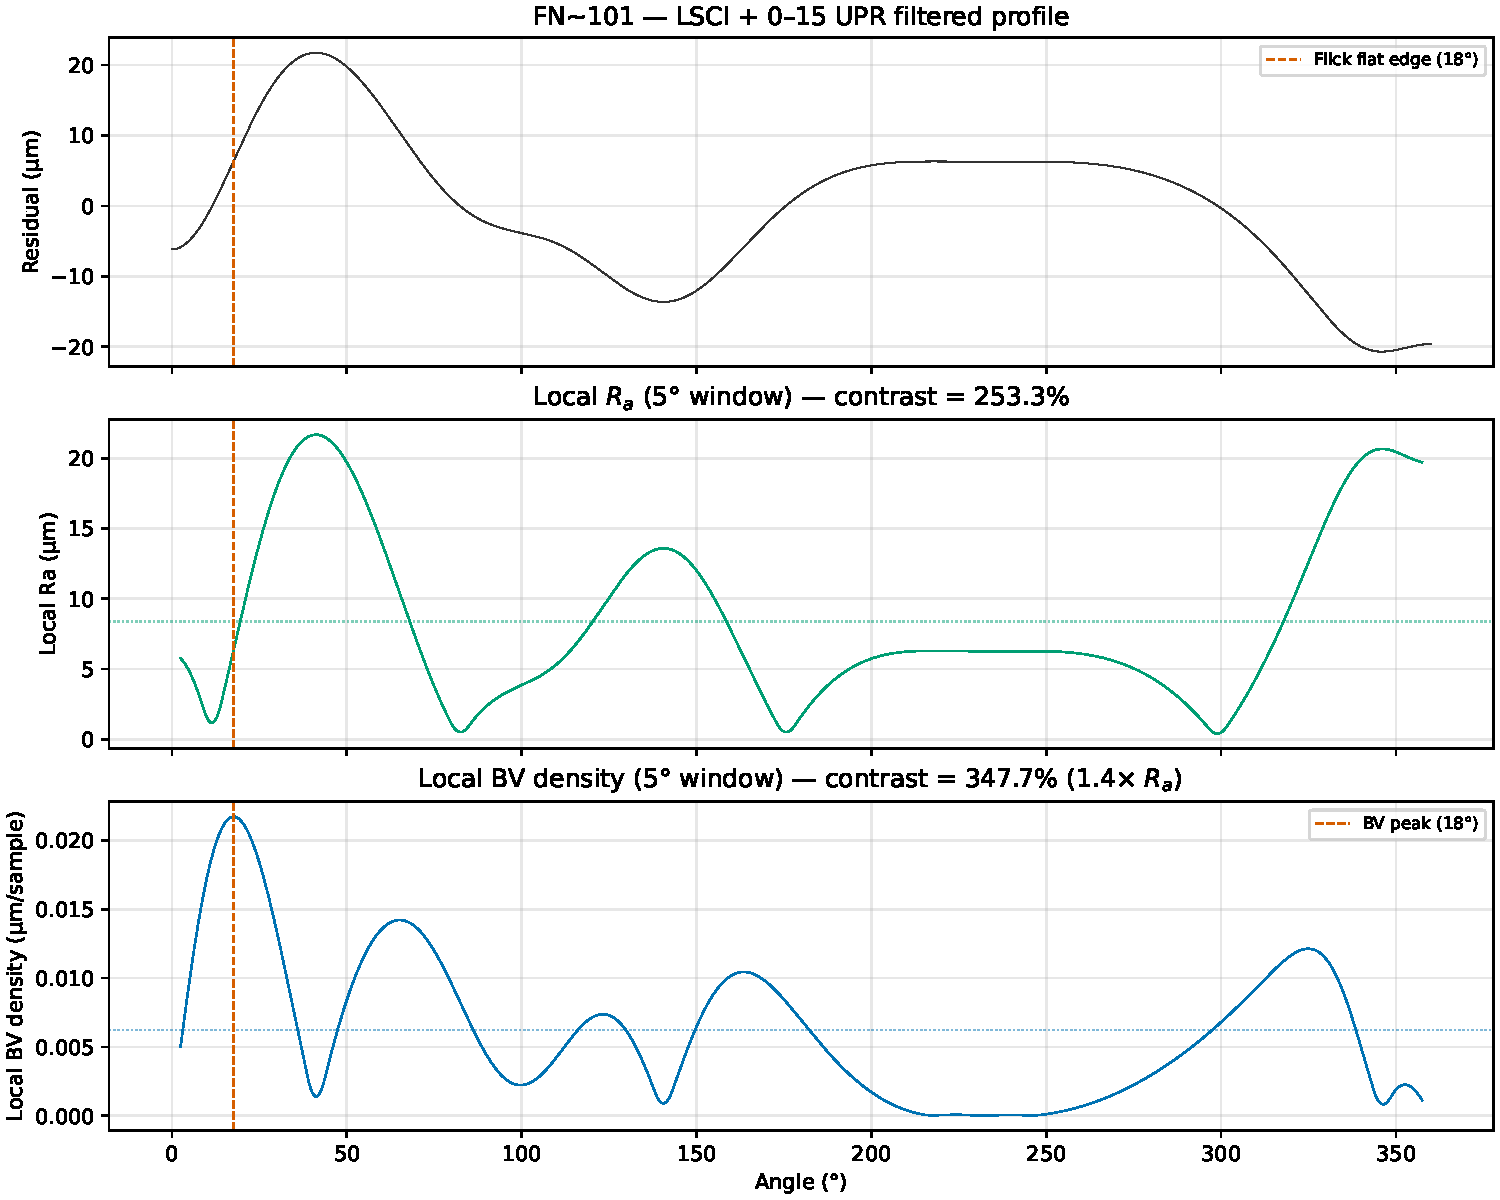
\includegraphics[width=\textwidth]{../../results/radial_profile_reconstruction_metric/flick_flat_detection.pdf}
\caption{Flick flat detection on the FN~101 magnification standard. BV density (bottom) shows a clear spike at the Flick flat angular position, whereas $R_a$ computed in a sliding window (top) shows no detectable response at the reconstruction resolution. The sliding-window width was matched to the certified angular extent of the Flick flat as specified in the DAkkS-DKD certificate (Art.~532~528); identical window parameters were used for both descriptors.}
\label{fig:flick_flat_detection}
\end{figure}

The Flick flat produces a clear response in BV density while showing no detectable response in a sliding-window $R_a$ analysis at the reconstruction resolution (Fig.~\ref{fig:flick_flat_detection}), illustrating the potential complementary sensitivity of gradient-based descriptors to localised geometric features.

\FloatBarrier
\section{Discussion}

\subsection{Confirmed Results}
The analysis rests on a key metrological distinction: an interferogram is an intensity measurement, not a phase map and not a height map. The half-wavelength relation $z=\nu\lambda/2$ becomes valid only after each image has been decoded to a wrapped excess fraction and the ordered excess-fraction sequence has been unwrapped to the continuous fringe-order coordinate $\nu$. This is why the reported comparison uses only reconstructed nanometre profiles, not raw greyscale images and not areal height maps.

The most sensitive part of the workflow is the EFM localisation of bright-ring maxima, with an excess-fraction uncertainty of approximately $\pm 0.05$ fringe orders (tightened to $\pm 0.03$ by sinusoidal refinement in $72\%$ of FN~111 frames). A single $\epsilon_i$ error of $0.05$ fringe corresponds to $13$~nm, sub-dominant to the $85$~nm residual-profile RMS. The chronological unwrapping criterion rejects phase jumps exceeding $0.35$ fringe. The median number of detected rings is three for both artefacts within the 240~px central aperture. The five $400^\circ$ ceramic sweeps require a geometric correction: successive useful $360^\circ$ intervals are shifted by $40^\circ$ because the physical object angle advances continuously; without this correction, the LSCI fit appears inconsistent even when phase extraction within each sweep is repeatable.

The linear drift of $0.0246$ fringe\,frame$^{-1}$ in the steel unwrapped phase sequence (versus $0.00021$ for the FN~111) is attributed to cumulative bias in the global unwrapping algorithm rather than thermal effects or axial runout~\cite{NewportCorporation:2018vk}.\label{sec:discussion_drift} The lower fringe contrast of the FN~101 interferograms — likely due to surface finish — reduces per-frame EFM quality; the pipeline applies automatic linear detrending where needed.

\subsection{Interpretation}

\subsubsection{Eccentricity removal and wobble verification}
\DIFaddbegin \label{sec:eccentricity}
\DIFaddend Roundness descriptors are computed after LSCI reference-circle fitting (Sec.~\ref{sec:topography}), which removes the first harmonic. A shared model across all five sweeps yields $R^2=0.99991$ with per-sweep amplitude variation of 63~nm ($0.18\%$); the manufacturer-specified wobble ($\pm 12~\mu$rad) bounds the observed variation an order of magnitude below $RONt=278$~nm. The polar representation (Fig.~\ref{fig:ceramic_roundness_polar}) shows five overlaid sweeps repeatable to $\pm 50$~nm, illustrating that the residual is dominated by low-order form deviation rather than random roughness.

\subsection{Comparison with ISO Parameters}
\label{sec:critical}

A central question of this work is whether gradient-based functional descriptors provide additional descriptive sensitivity alongside classical ISO parameters when applied to the same reconstructed profiles. To answer this rigorously, every descriptor was computed on the same reconstructed nanometre residual profiles.

\textbf{Mathematical equivalences.} The $L^1$ norm is defined as $\frac{1}{N}\sum|p_i-\bar{p}|$, which is identical to the definition of $R_a$. The $L^2$ norm is $\sqrt{\frac{1}{N}\sum(p_i-\bar{p})^2}$, identical to $R_q$. Computing both on the same centred residual yields \emph{exact numerical equality}: $R_a-L^1=0$ and $R_q-L^2=0$ to machine precision for both artefacts (Table~\ref{tab:metric_phase_reconstruction}). These equalities are not empirical findings; they are definitional consequences. Labelling the arithmetic mean of absolute deviations as $L^1$ rather than $R_a$ provides no new metrological information and should not be presented as a methodological advance.

It is emphasised that neither the $L^p$ norms nor the Sobolev and BV seminorms are presented as novel mathematical constructs; they are standard tools whose definitions are restated for completeness. Their value in the present context is threefold. First, the functional-analytic taxonomy places ISO parameters at specific positions ($L^1$, $L^2$, $L^\infty$) within a larger space of possible descriptors, revealing that descriptors outside the ISO set — BV density, $W^{1,2}$ seminorm — respond differently to the same perturbations. Second, the synthetic-defect injection methodology provides a controlled, like-for-like comparison framework that can be applied to any descriptor computed from the same residual profile; the framework itself, rather than any individual norm, constitutes the methodological contribution. Third, the Flick flat on the certified FN~101 standard provides a concrete existence proof: a real, DAkkS-DKD-certified artefact whose defining geometric feature is detected unambiguously by BV density while remaining below the detection threshold of sliding-window $R_a$ (Fig.~\ref{fig:flick_flat_detection}).

\textbf{Extrema: $R_z$ versus $L^\infty$.} $R_z/L^\infty \approx 2$ for both artefacts, consistent with symmetric positive and negative excursions. $L^\infty$ captures the single largest one-sided excursion; the ratio serves as a simple symmetry indicator.

\textbf{Variation-based descriptors.} A controlled sensitivity analysis (Supplementary Table~S2) examined five synthetic defect types injected into the FN~111 residual profile. Amplitude-averaging descriptors ($R_a$, $R_q$, $R_z$) showed no detectable change at the reconstruction resolution — a single $100$~nm spike changed $R_a$ by less than $0.05\%$, below the per-frame phase-extraction precision — while BV density increased by $+18\%$ and the $W^{1,2}$ gradient seminorm by $+622\%$ for the same spike (Fig.~\ref{fig:descriptor_sensitivity}). ISO shape parameters responded to asymmetry ($R_{sk}$ changed by $-1104\%$ for a step) but not to symmetric localised features. $R_{sk}$ and BV density appear complementary in the tested scenarios: $R_{sk}$ responds to asymmetry, BV density responds to localised gradients.

\DIFaddbegin \textbf{\DIFadd{Translation of synthetic responses to realistic defects.}} \DIFadd{The injected defects are idealised (isolated spike, uniform scratch, pure sinusoid), whereas real manufacturing defects have complex, random morphologies. The synthetic responses nevertheless translate to other backgrounds through a simple scaling argument. A localised defect adds a total-variation increment $\Delta TV$ that depends only on the defect geometry ($\Delta TV \approx 2A$ for an isolated spike of amplitude $A$), so the relative full-profile BV-density response is $\Delta TV / TV_{\mathrm{background}}$. On the FN~111 background ($TV=1.137~\mu$m) a 100~nm spike yields $+18\%$; on the FN~101 background ($TV=118.4~\mu$m) the identical spike would yield only $+0.17\%$, below the within-run repeatability. Detectability of a given absolute defect in the full-profile descriptor therefore scales inversely with the background gradient content, which quantifies the reviewer-relevant observation that the FN~101 defect-to-background ratio is roughly 500 times less favourable than typical smooth-surface applications. Two consequences follow for industrial inspection. First, full-profile BV density is best suited to smooth, finished surfaces — bearing raceways, optical components, precision seals — whose residual amplitudes (tens of nanometres) are comparable to the FN~111 case, and where the synthetic archetypes map onto realistic features (spike $\leftrightarrow$ pit or inclusion edge, scratch $\leftrightarrow$ handling or tooling mark, sinusoid $\leftrightarrow$ chatter or vibration signature). Second, for rougher backgrounds the sliding-window formulation restores local contrast: the certified Flick flat is detected on the FN~101 (Fig.~\ref{fig:flick_flat_detection}) despite the unfavourable full-profile ratio, precisely because the window localises the comparison. Validation against physical defects of calibrated dimensions on real metallic and ceramic surfaces remains necessary before these scaling arguments can be considered established (Sec.~\ref{sec:future}).
}

\DIFaddend \FloatBarrier
\begin{figure}[ht]
\centering
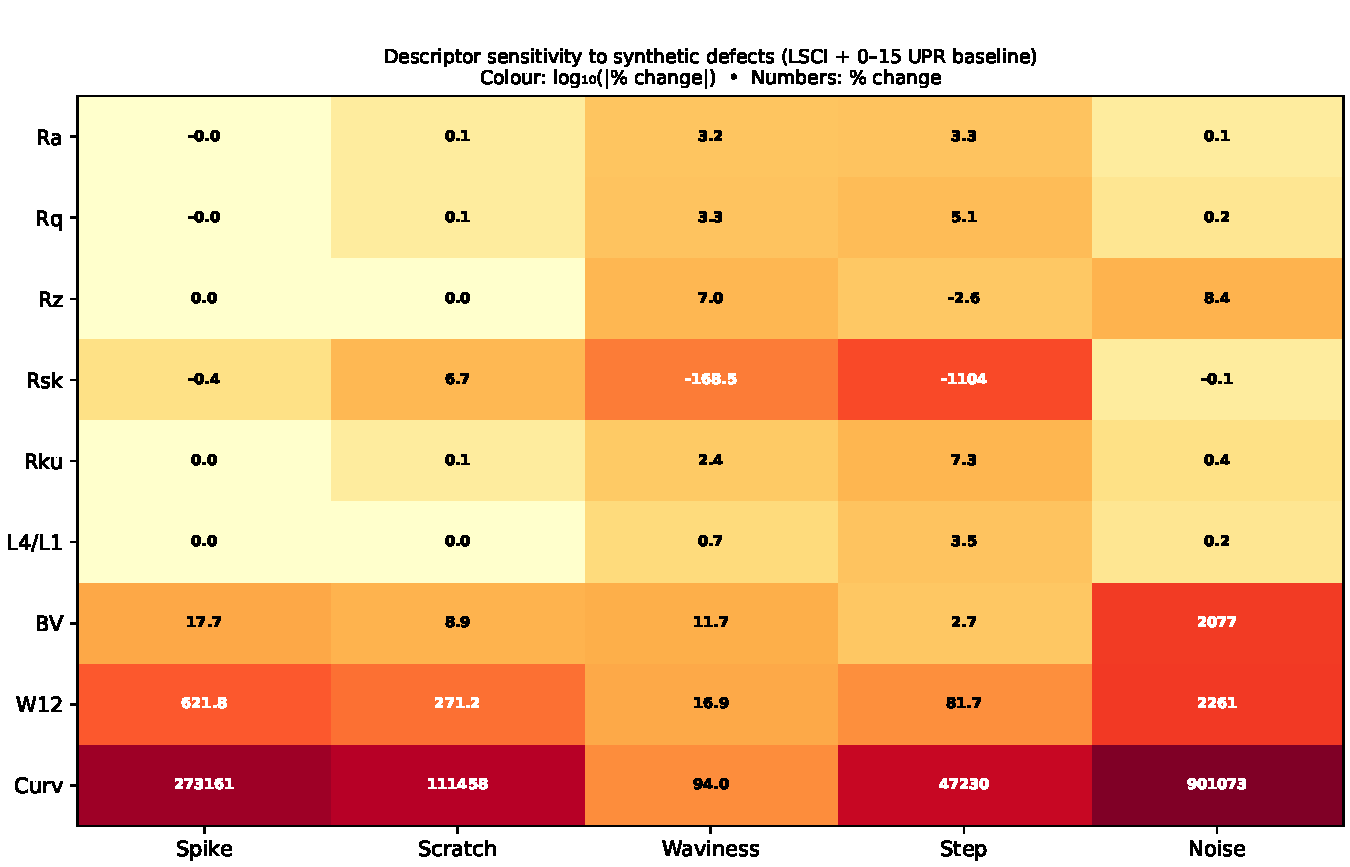
\includegraphics[width=0.95\textwidth]{../../results/radial_profile_reconstruction_metric/descriptor_sensitivity.pdf}
\caption{Sensitivity of ISO and gradient-based descriptors to five synthetic defect types injected into the FN~111 residual profile. Percentage change from the unperturbed baseline; bold labels indicate changes exceeding 10\%.}
\label{fig:descriptor_sensitivity}
\end{figure}

Supporting analyses — descriptor correlation matrices, power spectral density comparison, Cohen's $d$ effect sizes, critical descriptor assessment, and $L^p$ norm convergence — are provided in the Supplementary Materials (Figs.~S13--S17). Given the number of descriptors compared ($\sim$15 across two artefacts), the reported differences should be interpreted as exploratory rather than confirmatory; no formal multiple-comparison correction has been applied.

\textbf{Practical considerations.} A practical suggestion for interferometric profile and roundness metrology is to retain $R_a$, $R_q$, $R_z$, $R_{sk}$, $RONt$ and $RONq$ as the primary engineering layer compliant with ISO~\DIFdelbegin \DIFdel{4287}\DIFdelend \DIFaddbegin \DIFadd{21920-2}\DIFaddend , and to consider supplementing them with BV density (in angular units, nm\,deg$^{-1}$\DIFaddbegin \DIFadd{, Sec.~\ref{sec:angular_units}}\DIFaddend ) as a gradient-sensitive functional-analysis complement. The $W^{1,2}$ gradient seminorm is \DIFaddbegin \DIFadd{strongly }\DIFaddend correlated with BV density in the present datasets (within the FN~111: Pearson $r=0.95$, $n=5$ sweeps; within the FN~101: $r=0.93$, $n=5$). The pooled $r=0.94$ (95\% CI $[0.72,0.99]$, $n=10$) is reported for descriptive purposes only --- the sweeps are not independent observations and this pooled correlation should be interpreted with caution. \DIFaddbegin \DIFadd{This strong correlation indicates that, as }\emph{\DIFadd{repeatability metrics across sweeps}}\DIFadd{, BV density and the }\DIFaddend $W^{1,2}$ \DIFdelbegin \DIFdel{may add limited independent informationbeyond BV density alone given the small sample. The }\DIFdelend \DIFaddbegin \DIFadd{seminorm carry largely redundant information, and routine reporting of both is not warranted. They are strongly correlated but not mathematically equivalent: BV integrates the first power of the local slope, $TV=\int|p'|\,ds$, whereas $W^{1,2}$ integrates its square, $\int|p'|^2\,ds$, so the two coincide only for profiles whose slope magnitude is nearly constant and diverge whenever the slope distribution is uneven. This is exactly what the defect responses show: for the 100~nm synthetic spike the $W^{1,2}$ seminorm responded with $+622\%$ versus $+18\%$ for BV density, because the quadratic weighting amplifies a single steep event far more strongly than the linear total-variation measure. A practical reading of the descriptor space in these data is therefore: (i)~$R_a$/$R_q$ (equivalently $L^1$/$L^2$) carry amplitude information; (ii)~$R_{sk}$ carries an independent asymmetry axis; (iii)~BV density carries the localised-gradient axis and is recommended as the primary gradient descriptor; (iv)~the $W^{1,2}$ seminorm adds value mainly as a high-sensitivity alarm for isolated steep features rather than as an independent information axis; and (v)~the }\DIFaddend $L^4/L^1$ peakiness ratio provides a supplementary distribution-shape axis with a direct physical interpretation as the amplification of dominant profile excursions relative to $R_a$. These additional descriptors are computed from the same residual profile without additional hardware or changes to the EFM pipeline. The cross-instrument validation suggests that gradient-based descriptors are applicable to any 1D profile, whether from interferometry or tactile roundness measurement.

\DIFaddbegin \textbf{\DIFadd{Practical value and the known-feature caveat.}} \DIFadd{It must be acknowledged that the Flick flat is a certified, deliberately manufactured feature whose presence and position were known in advance: Fig.~\ref{fig:flick_flat_detection} is an existence proof under ground-truth conditions, not a blind detection study. The practical argument for a gradient-sensitive layer is therefore not that it revealed an unknown defect here. It is that it converts what an operator might notice in a visual polar-plot inspection into a quantitative, thresholdable, and automatable indicator computed from data already acquired for ISO reporting — with no operator in the loop, a defined angular position estimate, and a repeatability statement. Whether this indicator reveals defects that routine quality-control reporting would otherwise miss has not been demonstrated; a blind-detection protocol on artefacts with independently characterised defects is outlined in Sec.~\ref{sec:future} as the decisive next test of practical value.
}

\DIFaddend \textbf{Planned versus exploratory comparisons.} The synthetic-defect responses (Supplementary Table~S2, Fig.~\ref{fig:descriptor_sensitivity}) and the Flick flat detection (Fig.~\ref{fig:flick_flat_detection}) were planned comparisons motivated by the study's objective of assessing gradient-based descriptor sensitivity. The correlation matrices, power spectral density comparison, Cohen's $d$ effect sizes, $L^p$ norm convergence analysis, and the cross-descriptor stability comparison (Supplementary Figs.~S13--S17) are exploratory and are intended to characterise the descriptor space rather than to test specific hypotheses. This distinction should be borne in mind when interpreting the reported associations. The present study is a proof-of-concept demonstration; generalisability to other artefact types, materials, and measurement instruments remains to be established.

\subsection{Limitations}
Several limitations should be acknowledged. First, the uncertainty analysis \DIFdelbegin \DIFdel{is restricted to }\DIFdelend \DIFaddbegin \DIFadd{combines }\DIFaddend within-run Type~A repeatability from five sweeps\DIFdelbegin \DIFdel{in a single continuous rotation.}\DIFdelend \DIFaddbegin \DIFadd{, the indicative type-B budget of Sec.~\ref{sec:typeB} (including the measured static-session drift bound), and a two-session between-run comparison (Sec.~\ref{sec:between_run}) that shows agreement within combined uncertainties for identical acquisition parameters; a full multi-session reproducibility campaign with multiple independent setups and thermal cycles remains to be performed. }\DIFaddend The small $n=5$ limits statistical power (relative differences below $\sim30\%$ cannot be resolved \DIFdelbegin \DIFdel{), and between-run reproducibility (independent setups, thermal cycles, re-centring) has not been assessed. A full GUM-compliant uncertainty budget, incorporating type-B evaluations of laser wavelength stability, refractive-index variations, Abbe error, camera nonlinearity, and form-removal uncertainty, is beyond the scope of this study}\DIFdelend \DIFaddbegin \DIFadd{for the FN~111)}\DIFaddend ; the reported expanded uncertainties should be interpreted as lower bounds\DIFaddbegin \DIFadd{, and the form-removal systematic (bounded at $\leq41$~nm) is carried outside the quadrature combination}\DIFaddend .

Second, the validation is restricted to two artefacts from a single manufacturer (JENOPTIK), both \DIFaddbegin \DIFadd{of }\DIFaddend $\sim30$~mm diameter\DIFdelbegin \DIFdel{; }\DIFdelend \DIFaddbegin \DIFadd{. The two artefacts do differ substantially in material (Al$_2$O$_3$ ceramic versus steel) and in residual amplitude (two orders of magnitude in $R_a$), which provides some breadth, but }\DIFaddend generalisability to other \DIFdelbegin \DIFdel{sizes, materials , or }\DIFdelend \DIFaddbegin \DIFadd{diameters, materials such as optical glass or tungsten carbide, and other }\DIFaddend surface finishes has not been tested. Third, the synthetic-defect analysis uses idealised mathematical defects (isolated spike, uniform scratch, pure sinusoid) injected into the FN~111 ceramic profile only; the response to real manufacturing defects with complex morphologies may differ, and the \DIFdelbegin \DIFdel{defect-to-background ratio for }\DIFdelend \DIFaddbegin \DIFadd{scaling analysis of Sec.~\ref{sec:critical} shows quantitatively that full-profile detection sensitivity degrades in proportion to background gradient content (}\DIFaddend the FN~101 \DIFdelbegin \DIFdel{is approximately }\DIFdelend \DIFaddbegin \DIFadd{ratio is $\sim$}\DIFaddend 500 times \DIFdelbegin \DIFdel{smaller, so the detection sensitivity reported here may not generalise to artefacts with substantially larger form deviations}\DIFdelend \DIFaddbegin \DIFadd{less favourable)}\DIFaddend . Fourth, BV density and \DIFaddbegin \DIFadd{the }\DIFaddend $W^{1,2}$ seminorm carry intrinsic sampling-interval dependence\DIFdelbegin \DIFdel{requiring conversion to angular units for cross-instrument comparison.}\DIFdelend \DIFaddbegin \DIFadd{; the angular-unit convention of Sec.~\ref{sec:angular_units} standardises reporting, but no inter-laboratory evidence yet exists that the convention transfers across instruments. }\DIFaddend Fifth, the Flick flat result (Supplementary Fig.~S18) is demonstrated on a single artefact with a known\DIFaddbegin \DIFadd{, certified }\DIFaddend macroscopic feature; \DIFdelbegin \DIFdel{performance }\DIFdelend \DIFaddbegin \DIFadd{blind-detection performance and performance }\DIFaddend for subtler, micrometre-scale defects \DIFdelbegin \DIFdel{has }\DIFdelend \DIFaddbegin \DIFadd{have }\DIFaddend not been characterised.

\subsection{Metrological Implications}
The results carry several implications for profile and roundness metrology practice. The finding that BV density responds to localised gradients that amplitude averaging may not capture suggests --- subject to further validation --- a potential role for gradient-based descriptors in applications where isolated defects are of concern; possible examples include quality control of bearing surfaces, optical components, or precision seals. Because these descriptors are computed from the same residual profile used for ISO~\DIFdelbegin \DIFdel{4287 }\DIFdelend \DIFaddbegin \DIFadd{21920-2 }\DIFaddend parameters, their adoption does not require changes to existing measurement acquisition protocols.

The ISO~\DIFdelbegin \DIFdel{4287 framework }\DIFdelend \DIFaddbegin \DIFadd{21920-2 framework (with ISO~4287 as its predecessor) }\DIFaddend remains the appropriate baseline for surface texture specification and conformity assessment. The gradient-based descriptors discussed here are proposed as optional supplementary indicators, not as replacements for standardised parameters. Their metrological utility would be strengthened by inter-laboratory comparisons, by evaluation on a wider range of artefact types, and by \DIFdelbegin \DIFdel{the development of agreed procedures for converting sampling-dependent units to instrument-independent angular gradient units.}\DIFdelend \DIFaddbegin \DIFadd{adoption of the angular-unit reporting convention of Sec.~\ref{sec:angular_units}. }\DIFaddend Until such steps are taken, BV density and related descriptors should be regarded as research-grade tools whose diagnostic value has been observed under controlled laboratory conditions on two specific artefacts.

\subsection{Future Work}
\DIFaddbegin \label{sec:future}
\DIFaddend The present study suggests several directions for further investigation. (i)~A \DIFaddbegin \DIFadd{multi-session }\DIFaddend between-run reproducibility \DIFdelbegin \DIFdel{study }\DIFdelend \DIFaddbegin \DIFadd{campaign }\DIFaddend with independent setups\DIFdelbegin \DIFdel{and }\DIFdelend \DIFaddbegin \DIFadd{, distinct thermal cycles, and physical }\DIFaddend re-centring \DIFdelbegin \DIFdel{would establish whether the gradient-based descriptors retain their relative stability under realistic laboratory conditions.}\DIFdelend \DIFaddbegin \DIFadd{of the artefact would extend the two-session comparison of Sec.~\ref{sec:between_run} and would supply the input distributions needed to upgrade the indicative type-B budget of Sec.~\ref{sec:typeB} to a complete GUM-compliant evaluation. }\DIFaddend (ii)~Extending the validation to artefacts with different diameters, materials (e.g., \DIFdelbegin \DIFdel{glass, }\DIFdelend \DIFaddbegin \DIFadd{optical glass, tungsten }\DIFaddend carbide), and surface finishes would test the generalisability of the findings \DIFaddbegin \DIFadd{beyond the two $\sim$30~mm JENOPTIK artefacts studied here}\DIFaddend . (iii)~A systematic characterisation of BV density response to real manufacturing defects (scratches, pits, inclusions) of \DIFdelbegin \DIFdel{controlled dimensions}\DIFdelend \DIFaddbegin \DIFadd{calibrated dimensions, culminating in a blind-detection protocol in which the analyst does not know defect presence or position, }\DIFaddend would bridge the gap between the present synthetic-defect analysis and industrial inspection \DIFdelbegin \DIFdel{scenarios}\DIFdelend \DIFaddbegin \DIFadd{and would provide the decisive test of practical value}\DIFaddend . (iv)~An inter-laboratory comparison using a common artefact set and a standardised processing pipeline would provide the reproducibility data needed to assess whether BV density could eventually be considered for standardisation. (v)~\DIFdelbegin \DIFdel{The development of agreed }\DIFdelend \DIFaddbegin \DIFadd{Empirical verification of the }\DIFaddend angular-unit \DIFdelbegin \DIFdel{conventions for sampling-dependent gradient descriptors would facilitate cross-instrument comparison and potential inclusion }\DIFdelend \DIFaddbegin \DIFadd{convention of Sec.~\ref{sec:angular_units} across instruments with different angular resolutions would support the potential inclusion of gradient descriptors }\DIFaddend in reference software for roundness evaluation. \DIFaddbegin \DIFadd{(vi)~A systematic study of the speed--accuracy trade-off (rotation speed, frame rate, fringe contrast) would establish the shortest acquisition compatible with the reported uncertainty, a prerequisite for industrial adoption.
}\DIFaddend 

\section*{Data Availability}
The analysis code, processed results, and all figures are available at \url{https://github.com/dawidkucharski/banach-profile-metrology} (release v1.1.0). The raw interferometric PNG archives ($\sim$32~GB)\DIFaddbegin \DIFadd{, together with the two additional independent FN~111 sessions used for the between-run comparison of Sec.~\ref{sec:between_run} and the static stability recording used for the drift bound in Sec.~\ref{sec:typeB} ($\sim$7~GB each), }\DIFaddend are available from the corresponding author upon reasonable request.

\DIFdelbegin %DIFDELCMD < \bibliography{bib,scopus-banach,scopus-interfero}
%DIFDELCMD < %%%
\DIFdelend \DIFaddbegin \bibliography{bib}
\DIFaddend 

\end{document}
